\documentclass[12pt]{uthesis-v12}
\usepackage{graphicx}
\usepackage{amsmath}
\usepackage{listings}
\lstset{ %
  basicstyle=\footnotesize,       % the size of the fonts that are used for the code
  breakatwhitespace=false,        % sets if automatic breaks should only happen at whitespace
  breaklines=true,                % sets automatic line breaking
%  commentstyle=\color{rgb}{0,0.6,0},   % comment style
%  keywordstyle=\color{blue},      % keyword style
  language=Python,                % the language of the code
  numbers=left,                   % where to put the line-numbers; possible values are (none, left, right)
  numbersep=5pt,                  % how far the line-numbers are from the code
%  numberstyle=\tiny\color{gray},  % the style that is used for the line-numbers
%  rulecolor=\color{black},        % if not set, the frame-color may be changed on line-breaks within not-black text (e.g. comments (green here))
  showspaces=false,               % show spaces everywhere adding particular underscores; it overrides 'showstringspaces'
  showstringspaces=false,         % underline spaces within strings only
  showtabs=false,                 % show tabs within strings adding particular underscores
  stepnumber=1,                   % the step between two line-numbers. If it's 1, each line will be numbered
%  stringstyle=\color{mauve},      % string literal style
  tabsize=2,                      % sets default tabsize to 2 spaces
}
\begin{document}

%XXXXXXXXXXXXXXXXXXXXXXXXXXXXXXXXXXXXXXXXXXXXXXXXXXXXXXXXXXXXXXXXXXXX

\title{Amplified Total Internal Reflection at the Surface of Gain Medium}

\author{Josh Orndorff}
\copyrightpage{no} %only other option: yes

\mydocument{Thesis} %Other Option: Project, Dissertation
\degree{Masters of Science}{Physics} %Section 3.4 of Read_Me_First_(v12).pdf

\conferraldate{May}{2013}
\advisor{Dr.~Victor Karpov}
\secondmember{Dr.~Brian Bagley}
\thirdmember{Dr.~Robert Deck}
% \fourthmember{Dr.~Adam Baum}
% \fifthmember{Dr.~Corey O.~Graff}
\graduatedean{Dr.~Patricia R.~Komuniecki}{Dean}

\maketitle

%XXXXXXXXXXXXXXXXXXXXXXXXXXXXXXXXXXXXXXXXXXXXXXXXXXXXXXXXXXXXXXXXXXXX

\begin{abstractpage}
Total Internal Reflection (TIR) is the phenomenon whereby a light wave incident on a boundary is completely reflected when the wave's incidence angle exceeds a critical angle, $\theta_c$. For decades there has been debate about whether amplified TIR from a medium exhibiting optical gain is possible, and desire for a theory to explain it. Authors have suggested theories both in favor and in doubt of the phenomenon's existence, and experimental evidence has arose supporting the existence and seemingly simultaneously contradicting proposed theoretical models. In this thesis, reflection coefficients for plane waves are calculated by satisfying boundary conditions from Maxwell's equations at the reflecting surface for both optically lossy and gainy media. Plane wave reflectivity is found to exhibit is discontinuous jump from below unity to above as the incidence angle passes through the critical angle, confirming the existence of amplified TIR. Fourier analysis is used to show that finite beams also exhibit amplified TIR, but do not experience the surprising discontinuous jump in reflectivity at the critical angle.
\end{abstractpage}

%XXXXXXXXXXXXXXXXXXXXXXXXXXXXXXXXXXXXXXXXXXXXXXXXXXXXXXXXXXXXXXXXXXXX

%\begin{dedication}
%\noindent [Insert your dedication here]
%\end{dedication}

%XXXXXXXXXXXXXXXXXXXXXXXXXXXXXXXXXXXXXXXXXXXXXXXXXXXXXXXXXXXXXXXXXXXX

\begin{acknowledgments}
\noindent
Foremost, I would like to thank Dr. Robert Deck for his unceasing insight, patience, encouragement, and desire to help. I also thank the rest of my committee, Dr. Victor Karpov and Dr. Brian Bagley, for their support of my work. Another thanks goes to my classmates at the university for the time they spent proofing my work, arguing about various physics concepts, and motivating me to keep working hard. In particular, I'd like to thank Joseph Booker for his help with python programming, Aditya Togi, for his help with analytical mathematics, and Alex Cimaroli and Max Junda for their encouragement and helpful suggestions both academically and socially.

I'm also grateful to my family for their support and encouragement throughout my school career. And, finally, I'd like to acknowledge the contributions from the authors, contributors, and supporters of the open-source projects NumPy and Matplotlib. Without their code, I could never have completed the numerical calculations contained herein.
\end{acknowledgments}

%XXXXXXXXXXXXXXXXXXXXXXXXXXXXXXXXXXXXXXXXXXXXXXXXXXXXXXXXXXXXXXXXXXXX

\tableofcontents  %----->  DO NOT ALTER THIS COMMAND
%\listoftables     % If three or more tables
\listoffigures    % If three or more figures

\captionformat{hang}
%\captionformat{align}


%XXXXXXXXXXXXXXXXXXXXXXXXXXXXXXXXXXXXXXXXXXXXXXXXXXXXXXXXXXXXXXXXXXXX

\begin{listofabbreviations} %Optional
 \abbreviation{TIR}{Total Internal Reflection -- When a plane wave is completely reflected from a boundary.}
 \abbreviation{aTIR}{Attenuated Total Internal Reflection -- TIR wherein the reflected beam is less intense than the incident beam.}
 \abbreviation{ATIR}{Amplified Total Internal Reflection -- TIR wherein the reflected beam is more intense than the incident beam.}
 \abbreviation{DFT}{Discrete Fourier Transform.}
 \abbreviation{FFT}{Fast Fourier Transform -- A time efficient algorithm for calculating the DFT.}
 \abbreviation{GH Shift}{Goos-Hanchen shift. The amount by which a reflected beam is shifted across a boundary from that predicted by geometrical optics.}
 \abbreviation{FDTD}{Finite difference time domain. A numerical method for solving differential equations including Maxwell's equations.}
\end{listofabbreviations}

%XXXXXXXXXXXXXXXXXXXXXXXXXXXXXXXXXXXXXXXXXXXXXXXXXXXXXXXXXXXXXXXXXXXX

\begin{listofsymbols}
%Lowercase English
 \emblem{$c$}{Light's speed in free space. $c=2.998 \,\mathrm{m/s}$}
 \emblem{$e$}{Euler's constant. $e \approx 2.71828$}
 \emblem{$i$}{The imaginary constant. $i \equiv \sqrt{-1}$}
 \emblem{$k$}{Wave number of an electromagnetic wave. $k=n\frac{2\pi}{\lambda}=n\frac{\omega}{c}$}
 \emblem{$\mathbf{k}$}{Wave vector. This vector's magnitude is the wave number, and its direction is the wave's propagation direction.}
 \emblem{$k_i$}{Wave number specifically for an incident wave. Subscripts r (reflected) and t (transmitted) are also used.}
 \emblem{$\tilde{k}_{tz}$}{Complex-valued wave number for a transmitted beam's $z$-component.}
 \emblem{$k_m$}{$k$-domain's $m^{th}$ sample in a discrete Fourier transform.}
 \emblem{$n_1$}{Real-valued refractive index characterizing the medium from which light is incident on a boundary.}
 \emblem{$\tilde{n}_2$}{Complex-valued refractive index characterizing the medium into which light is transmitted, or from which it is reflected. $\tilde{n}_2 = n_2 -i\gamma$}
 \emblem{$n_2$}{Real part of $\tilde{n}_2$. Characterizes the propagation of light in medium two.}
 \emblem{$\tilde{r}$}{Amplitude reflection coefficient for wave incident on a boundary. $\tilde{r} \equiv E_r/E_0$}
 \emblem{$w$}{Width of a Gaussian beam. The radial distance away from the center of the beam at which the light's intensity has fallen off by a factor of two.}
 \emblem{$w_0$}{Waist of a Gaussian beam. The width of the beam at its narrowest point.}
 \emblem{$\mathbf{x}$}{Position vector of components $x$, $y$, and $z$, in the 3D space spanned by $\hat{x}$, $\hat{y}$, and $\hat{z}$. The boundary is defined by the plane $z=0$.}
 \emblem{$\mathbf{x}'$}{Position vector in the coordinate system of a Gaussian beam. The beam propagates along the $z'$ direction.}
 \emblem{$x_n$}{$x$-domain's $n^{th}$ sample in a discrete Fourier transform.}
      \emblemskip

%Capital English
 \emblem{$\mathbf{D}$}{Electric displacement vector.}
 \emblem{$\mathbf{D}_i$}{Electric displacement field vector of incident plane wave. Subscripts $r$ (reflected) and $t$ (transmitted) are also used.}
 \emblem{$\mathbf{E}$}{Electric field vector.}
 \emblem{$\mathbf{E}_i$}{Electric field vector of incident plane wave. Subscripts $r$ (reflected) and $t$ (transmitted) are also used.}
 \emblem{$E_n$}{$n^{th}$ $x$-domain electric field sample in a discrete Fourier transform.}
 \emblem{$F_m$}{$m^{th}$ $k$-domain electric field sample in a discrete Fourier transform.}
 \emblem{$L$}{Spacial sampling interval in a discrete Fourier transform. $L=1/\kappa_s$.}
 \emblem{N}{Total number of samples (both spacial and wave number) in a discrete Fourier transform.}
 \emblem{$R$}{Intensity reflection coefficient. $R=\tilde{r}^*\tilde{r}$.}
       \emblemskip
       
%Greek
 \emblem{$\gamma$}{Imaginary part of $\tilde{n}_2$. Characterizes the absorption ($\gamma < 0$) or amplification ($\gamma > 0$) of light in medium two.}
 \emblem{$\epsilon_1$}{Real-valued permittivity characterizing the medium from which light is incident on a boundary.}
 \emblem{$\tilde{\epsilon}_2$}{Complex-valued permittivity characterizing the medium into which light is transmitted or from which it is reflected. $\tilde{\epsilon}_2\equiv\epsilon_2'+i\epsilon_2''$}
 \emblem{$\epsilon_2'$}{Real part of $\tilde{\epsilon}_2$. Characterizes the propagation of light in medium two.}
 \emblem{$\epsilon_2''$}{Imaginary part of $\tilde{\epsilon}_2$. Characterizes the absorption ($\epsilon_2''>0$) or amplification ($\epsilon_2''<0$) of light in medium two.}
 \emblem{$\theta_c$}{Critical angle of TIR}
 \emblem{$\theta_i$}{Incidence angle of a plane wave on a boundary.}
 \emblem{$\theta_r$}{Reflection angle of a plane wave from a boundary.}
 \emblem{$\tilde{\theta_t}$}{Transmission angle of a plane wave (or Gaussian beam's central ray) from a boundary. $\tilde{\theta_t}$ is complex valued except when no gain or loss is present in medium two.}
 \emblem{$\theta_p$}{The incident angle necessary to excite a surface plasmon.}
 \emblem{$\kappa_s$}{Spacial sampling wave number in a discrete Fourier transform. $\kappa_s=1/L$}
 \emblem{$\lambda$}{Wavelength of a plane wave}
 \emblem{$\mu$}{Magnetic permeability of a medium. In this thesis all media are assumed to be non-magnetic. $\mu=1$ in Gaussian units or $\mu=\mu_0$ in SI units.}
\emblem{$\phi$}{Incidence angle of the central ray in a Gaussian beam.}
 \emblem{$\xi$}{Gouy phase of a Gaussian beam. $\xi\equiv\arctan z'/z_R$.}
 \emblem{$\omega$}{Angular frequency of a light wave.}

\end{listofsymbols}

\makebody   %------->  DO NOT ALTER THIS COMMAND

%XXXXXXXXXXXXXXXXXXXXXXXXXXXXXXXXXXXXXXXXXXXXXXXXXXXXXXXXXXXXXXXXXXXX

\chapter{Background and Motivation}\label{chap-intro}

Like all original research, this thesis builds on several ideas that have been previously established in optics.  In this introduction, I will summarize the relevant work that has already been done, illustrate and exemplify the debate that has surrounded the single surface amplified total internal reflection phenomenon, and very briefly outline the research presented in subsequent chapters.

\section{Total Internal Reflection}\label{intro-TIR}

The phenomenon of total internal reflection (TIR) has been well known for centuries. It can be observed in everyday life and is well understood theoretically\cite{Hecht}. When a wave is incident on a boundary surface, some of its energy, in general, is reflected back from the boundary, and some of its energy is transmitted into the second medium behind the boundary. The fact that boundary conditions exist means there are spacial and temporal constraints that lead to kinematic properties such as the law of reflection which states the reflection angle must be equal to the incident angle, $\theta_i=\theta_r$, and Snell's law which gives the transmission angle as $\sin\theta_t = \frac{n_1}{n_2}\sin\theta_i$, where $n_1$ and $n_2$ are the refractive indices of both media. Both of these laws will be re-derived in chapter \ref{chap-planeWaves} and will prove to be unaffected by the presence of gain or loss in the second medium.

The angle at which the right hand side of Snell's law exceeds one is known as the critical angle, denoted $\theta_c$. At this angle when TIR first occurs, no wave exists in the second medium whatsoever.  Beyond the critical angle, TIR continues to occur, but an evanescent, or exponentially decaying, wave is excited in the second medium. It is this evanescent wave that is responsible for the Goos-Hanchen shift (GH shift)\cite{Fan}.

\begin{figure}[ht]
 \centering
 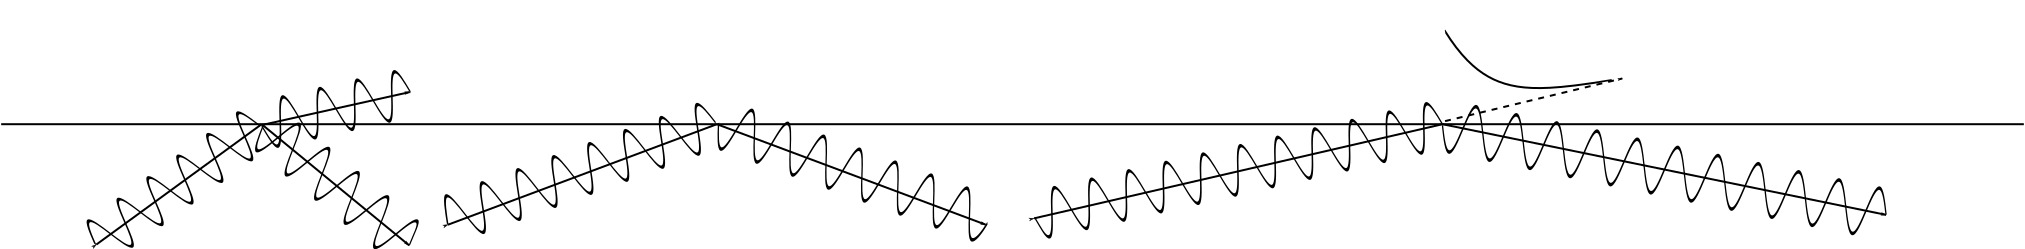
\includegraphics[width=1\textwidth]{diagrams/fig-TIRDiagram.eps}
 \caption[Light incident on a lossless boundary above and below the critical angle.]{Light incident on a lossless boundary above and below the critical angle. Left - Below the critical angle both a reflected and transmitted beam exist. Middle - At the critical angle only a totally reflected beam exists. Right - Beyond the critical angle a totally reflected beam and an evanescent field exist.
 \label{fig-TIRDiagram}}
\end{figure}

In addition to the kinematic properties, the specific nature of the boundary conditions provides a set of dynamic equations, which define certain Fresnel coefficients describing the relative brightness of the reflected and transmitted waves. The Fresnel coefficients for lossless media are derived in most entry level optics texts \cite{Hecht} \cite{Jackson}, and will be re-derived in chapter \ref{chap-planeWaves}. Unlike the law of reflection and Snell's law, we will see that the Fresnel coefficients do change with the presence of gain or loss in medium two (sometimes in unintuitive and surprising ways ex. fig \ref{fig-lossyReflectivity}).

\begin{figure}[htb]
 \centering
 \includegraphics[width=1\textwidth]{plots/fig-losslessReflectivity.eps}
 \caption[Reflectivity from a lossless boundary.]
         {The plot shows intensity reflection coefficient, $R$, for plane waves from a boundary where both media are lossless. Note that the reflectivity is 100\% for all angles beyond the critical angle, but never exceeds 100\%.
 \label{fig-losslessReflectivity}}
\end{figure}

Practical applications of TIR are numerous. In the science lab, Abbe refractometry is used to determine refractive indices. In daily life, communication and data transfer happens largely over fiber optic cables which make use of TIR. Consequently a thorough theoretical understanding of all its manifestations is warranted.

The classical treatment discussed above is sufficient to describe the TIR phenomenon in cases of nearly transparent media, and incident beams that are not narrowly focused. The most useful results such as the critical angle, law of reflection and Snell's law are important enough that they are taught as part of most introductory physics courses. But the treatment above does not treat all physical properties of a real-world system, and is therefore incomplete.  Our understanding of total internal reflection can be made more robust by extending our model to correct for at least two deficiencies in the usual derivation.

First, the classical treatment assumes all media are perfectly transparent and  lossless.  In reality the vast majority of media, and certainly the media that we interact with everyday, such as glass, air, water, etc.~are all lossy, meaning they absorb some of the light that passes through them.  And some media such as laser dyes and other active media with inverted atomic populations are active or gainy, meaning they amplify the light that passes through them.  The lossy or gainy nature of such media can be accounted for by introducing a complex refractive index, $\tilde{n}=n-i\gamma$. This complex refractive index will be used in chapter \ref{chap-planeWaves} and throughout the remainder of the thesis. The extent to which these media absorb or amplify light depends on the frequency of light in question, so that in general $\tilde{n}=\tilde{n}(\omega)$, but the theory can be developed for a single frequency with the refractive index, $\tilde{n}$, taken to be a constant.

Second, the classical treatment assumes that both the incident plane wave and the boundary extend infinitely in directions perpendicular to the incidence plane.  More generally, edge effects  occur whenever either the beam or the boundary terminates, as they must in the real world. But in practice a laser beam with a width more than a dozen wavelengths incident on a boundary of more than a dozen beam widths can be well approximated as an infinite plane wave. Finite size effects become especially important when the beam width is on the order the incident light's wavelength.\cite{Konopsky}

This thesis will begin by re-deriving the Fresnel reflection coefficients for a second medium with gain or loss (focusing primarily on gain), and will discuss the significance of the results, considering the effects of both gain in layer two and finite beam width.

\section{Lasers and Gain Media}\label{intro-lasersAndGain}
The discovery of stimulated emission led to many advances in our understanding of optics as well as our ability to manufacture useful optical devices. By exciting media in clever ways so that their populations are in a non-thermal state where a majority of atoms are excited, known as population inversion, a gain medium is achieved such that stimulated emission will amplify light that passes through the gain medium.

\begin{figure}[ht]
 \centering
 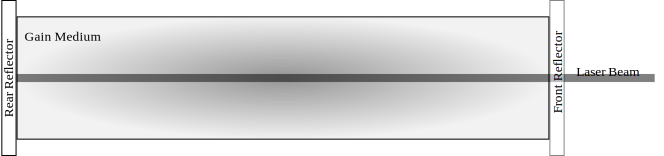
\includegraphics[width=\textwidth]{diagrams/fig-laserDiagram.eps}
 \caption[Internal structure of a laser.]
         {As light propagates through the gain medium in a laser, it is amplified via stimulated emission and a laser beam is produced.
 \label{fig-laserDiagram}}
\end{figure}

The laser cavity depicted above results in the emission of a narrowly focused, approximately Gaussian Intensity profile. Without the narrow beam of a laser, many of the TIR applications listed previously, as well as the experimental work outlined in section \ref{intro-experiments} would be impossible.

This thesis investigates theoretically the case where no wave propagates in a gain medium, but rather an evenescent wave exists in the gainy region.  It will also discuss the details of a Gaussian laser beam in chapter \ref{chap-finiteBeam} and use the formalization to predict real-world experimental results where only a finite beam (such as a Gaussian) can be realized.

\section{Amplified and Attenuated TIR}
Amplified total internal reflection (ATIR) is the phenomenon whereby a wave reflected from a boundary is more intense than the incident wave.  In the classical treatment above, this is clearly not possible as it would violate energy conservation. But as we know the treatment above is not the whole story.

Returning to the case of two semi-infinite media, and a plane boundary between them, we consider the case of a lossy second medium. It is established \cite{Fan} \cite{Willis} that attenuated total internal reflection occurs in this case, and the reflection coefficients will be derived in chapter \ref{chap-planeWaves}.  

\begin{figure}[ht]
 \centering
 \includegraphics[width=1\textwidth]{plots/fig-lossyReflectivity.eps}
 \caption[Attenuated reflectivity from a lossy boundary.]
         {P-state intensity reflection coefficients, $R$, for plane waves from a boundary where both media are lossless (red) and where medium two is lossy (blue). It is worth noting that reflectivity below the critical angle is actually higher in the lossy case despite loss in medium 2.
 \label{fig-lossyReflectivity}}
\end{figure}

The existence of such attenuated reflection begs the question whether amplified reflection could exist if the second medium were gainy rather than lossy.  The existence of an amplified total internal reflection would serve as a nice counterpart to this attenuated total internal reflection, but as we will see in section \ref{planeWaves-differentQuadrants}, there is a mathematical curiosity that has caused some authors to doubt its existence.

\subsection{Amplified TIR with Surface Plasmons}
To lend further credence to the idea of ATIR from a single gain medium boundary, it was shown\cite{Plotz} that enhanced reflection is theoretically possible if a thin metal film is inserted between the two media and the incidence angle is near that necessary to excite a surface plasmon, $\theta_i=\theta_p > \theta_c$.

Using modified Fresnel reflection coefficients similar to those derived in sections \ref{planeWaves-r} and \ref{planeWaves-R} the authors of \cite{Plotz} show that after the gain exceeds a certain threshold value, reflectivity is resonantly enhanced for incident angles in the vicinity of the plasmon angle, $\theta_i\approx\theta_p$. The authors also estimate that such enhanced reflection could be experimentally achievable in the near infrared using metals and gain media that could be practically manufactured.

\subsection{Some Interesting Experiments}\label{intro-experiments}
In 1966 Charles J.~Koester of the American Optical Company published a concise report detailing experimental results that he had achieved. His research team had previously had success transmitting and amplifying light through a fiber optic cable with a gainy core \cite{FiberExperiment}. They referred to such devices as ``active core fiber lasers". The devices transmitted light via TIR in the same way as a traditional fiber optic cable, but also amplified the light as it traveled.  In a later experiment Koester returned to a traditional passive core, and instead used an active cladding. In this case he again found that light was amplified as it traversed the fiber despite experiencing TIR from the cladding.  He interpreted this result to mean that light was reflected from the cladding with reflectivity greater than one. We will see in the following section that some authors have argued that Koester misinterpreted his results, but I will ultimately support his conclusion.

In 1972 a group of Soviet scientists, Kogan, Volkov, and Lebedev, performed an experiment at the Institute of Organic Semiconductors and Dyes showing that ATIR was possible with a single reflection from a planar surface \cite{Kogan1}. The report is sparcely quantitative, but they do report an intensity reflectivity of 25. The following year, the same group published a follow-up experiment reporting a single reflection gain of roughly 1000\cite{Kogan2}.

These two experiments, both of which demonstrate amplified reflection without surface plasmon coupling appear to further substantiate the intuitive thought that, if lossy media cause attenuated reflection, then gainy media may lead to amplified reflection.

\subsection{Amplified TIR with Gain Media}
Despite the experimental evidence discussed in the previous section, the mathematical results discussed in section \ref{planeWaves-differentQuadrants} still lead authors to support drastically different physical interpretations of the ATIR phenomenon.

The first theory attempting to explain amplified total internal reflection came just months after Kogan et. al.'s experiment was published. In September 1972 two Soviet theorists, Romanov and Shakhidzhanov published their work explaining ATIR using complex refractive indices and well known boundary conditions at the reflecting surface \cite{Romanov}. Their work was consistent with the sparse experimental data available at the time, and is the basis for much subsequent theoretical work including this thesis.

Just a few more months after Romanov and Shakhidzhanov published their theory, Kogan et. al. published the results of their second experiment \cite{Kogan2}. Their purported single pass gain of roughly 1000 was inconsistent with the recently published theory of Romanov and Shakhidzhanov.  Two years later a new theory came from two American authors at the University of Maine. Callary and Carniglia derived a new theory that was distinct from the Romanov and Shakhidzhanov theory in two important ways. First they treated a three layer problem where the gain medium was of finite thickness between two transparent half spaces. Their results regarding the two layer problem came from taking the limit as $d\to\infty$ for their gain slab. Second, they chose the complex conjugate wave vector for the transmitted beam (discussed in detail in section \ref{planeWaves-differentQuadrants}) which resulted in gain at all angles both above and below the critical angle. Their new theory appeared to be in agreement with the new experimental data, and allowed for arbitrarily high reflectivity (even allowing it to be infinite) for the correct combinations of layer thickness and incident angle.

In 1978, Plotz et. al. from the University of Toledo showed theoretically that enhanced reflectivity can be achieved when a thin metal layer is placed between the incident medium and the gain medium if the incidence angle is chosen to excite a surface plasmon on the metal surface \cite{Plotz}. Although treating a somewhat different problem, the results, like those of Callary and Carniglia, allowed for arbitrarily high (even infinite) reflectivity for the appropriate incidence angle and metal layer thickness. These results lend support to the Callary and Carniglia theory because they validate the surprising result of infinite gain.

Decades later in 2003, Fan et. al. revisited the topic of single surface ATIR and built on the work of R and S to calculate the Goos Hanchen shift (GH shift) for plane waves incident on a gainy medium \cite{Fan}. They made the same argument as presented in the original R and S paper to conclude that ATIR was possible beyond the critical angle but not below it.  Although they cited Callary and Carniglia to support their claim that ATIR was possible beyond the critical angle, they concluded that Callary and Carniglia were incorrect in stating that ATIR was possible at all angles. They did not offer an alternative explanation for Kogan et. al.'s measured gain of 1000.

Willis et. al. continued building on the theory of R and S and treated the important case of finite width beams theoretically for the first time \cite{Willis} in 2008. They elegantly showed both analytically and via finite difference time domain (FDTD) simulations that a finite width beam will exhibit ATIR beyond the critical angle, but will not experience the surprising discontinuity that plane waves do. However they, like Fan et. al., still did not account for the gain of 1000 that Kogan et. al. reported.

In 2011 a manuscript by Tobias and Masud Mansuripur attempted to explain all the experimental data, possibly including Kogan et. al.'s gain of 1000 result, using an entirely different interpretation of the theory \cite{Mansuripur}. Taking the exact opposite route from Callary and Carniglia, the Mansuripurs suggested that single surface ATIR was not possible at any angles, and claimed that reflection from lossy or gainy media was always less than one.  They argued that the observed amplification was in fact not due to reflection from the front surface of the material, but was observed because in all real experimental setups the gainy region is of finite thickness. They proposed that the observed amplification was due to a transmitted wave propagating through the gainy slab, partially reflecting from its back face, and propagating back to the front face.  Their manuscript was not accepted for publication, but was received as part of a private communication on the matter.

The history of this problem is long and interesting, with a revival in the literature in recent years. Proposed theoretical models range from Callary and Carniglia who conclude that ATIR is possible at all incident angles, to the Mansuripurs who claim that it is not possible at any angles. In section \ref{planeWaves-differentQuadrants}, I will discuss in detail the mathematical results that lead to this debate.

\section{Thesis Outline}
In the next chapter I will set up a standard coordinate system, define the variables and conventions used throughout this thesis, and derive the Fresnel reflection coefficients from Maxwell's equations.  I will then discuss and interpret the two possible mathematical solutions that led to the debate previously discussed, and show that the mathematical solution that leads to amplified total internal reflection is the physically correct solution.

In chapter \ref{chap-finiteBeam}, I will build on the results of chapter \ref{chap-planeWaves} to treat the reflectivity of finite width laser beams and investigate interesting edge effects that emerge when the beam  is only a few wavelengths wide.  I will also compare and evaluate the various numerical and analytical methods for performing such analyses. In the final section, I will consider the effect on the enhanced reflectivity produced by changes in various parameters of the system, such as refractive indices, gain, beam focus, polarization, and incident angle, and will discuss the significance of these results.

Finally, in chapter \ref{chap-conclusions}, I will summarize the detailed conclusions from throughout the text and emphasize their importance.

%XXXXXXXXXXXXXXXXXXXXXXXXXXXXXXXXXXXXXXXXXXXXXXXXXXXXXXXXXXXXXXXXXXXX

\chapter{Case of Incident Plane Waves}\label{chap-planeWaves}
In this chapter I establish the geometry and naming conventions followed throughout the thesis and use them to re-derive the Fresnel plane wave reflection coefficients for the case where the second medium is gainy or lossy.  I also discuss the slight differences that arise when treating p and s polarization of incident light.  Finally in section \ref{planeWaves-differentQuadrants} I resolve the various interpretations of the mathematics that have led to dispute about the existence of single surface amplified total internal reflection.

\section{Geometry and Boundary Conditions}
\begin{figure}[ht]\label{fig-rayGeometryDiagramP}
\centering
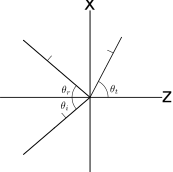
\includegraphics[width=.8\textwidth]{diagrams/RayGeometryDiagramP.eps}
\caption[Geometry for p polarization.]{Geometry for p polarization. Large arrows represent propagation direction of plane waves. Small arrows are direction of electric fields.
 \label{planeWaves-definitions}}
\end{figure}

The problem addressed in this thesis is fundamentally a two layer problem; its geometry is depicted in figure \ref{fig-rayGeometryDiagramP}. The boundary lies in the $z=0$ plane and the incidence plane is given by $y=0$. The medium on the left is transparent (neither lossy nor gainy) and characterized by the real-valued refractive index $n_1$. It is home to the incident wave which strikes the boundary at incident angle $\theta_i$ relative to its normal, and the reflected wave which is reflected back into the same medium at a reflection angle $\theta_r$.  The medium on the right is home to the transmitted wave which is refracted from the boundary at transmission angle, $\theta_t$ and is characterized by complex refractive index, $\tilde{n}_2=n_2-i\gamma$. The gain factor is called $\gamma$, and the explicit negative sign in the definition means that positive gamma is gainy and negative gamma is lossy. All quantities that are known to be complex will be explicitly indicated as such by the presence of a tilde over their variables, as is the case with $\tilde{n}_2$. Having specified the media's refractive indices, their permittivities can be calculated as $\epsilon_1=n_1^2$ and $\tilde{\epsilon}_2=\tilde{n}_2^2$.

In figure \ref{fig-rayGeometryDiagramP} the long rays indicate the direction in which waves are traveling. As is standard, wave vectors, $\mathbf{k}$, will point in the direction of propagation of their respective waves, and their magnitudes will be given by $k=n\frac{\omega}{c}$. The short arrows adjacent to each ray indicate the direction of the $\mathbf{E}$-field for each wave.  With these geometry conventions established, the wave vectors and fields of each wave can be written explicitly.

\begin{subequations}\label{eq-waveVectors}
\begin{equation}
k_i=k_r=n_1\frac{\omega}{c}
\end{equation}
\begin{equation}
\tilde{k}_t=\tilde{n}_2\frac{\omega}{c}=k_t-i\gamma\frac{\omega}{c}
\end{equation}

Note the definition of $k_t$ (without a tilde) in the immediately preceding equation.
\end{subequations}
\begin{align}\label{eq-waveformsP}
\mathbf{E}_i(\mathbf{x},t)&=E_{0i}(\cos\theta_i\mathbf{\hat{x}}-\sin\theta_i\mathbf{\hat{z}})
e^{i(k_{ix}x+k_{iz}z-\omega t)} \\ \label{eq-waveformsPr}
\mathbf{E}_r(\mathbf{x},t)&=E_{0r}(\cos\theta_r\mathbf{\hat{x}}+\sin\theta_r\mathbf{\hat{z}})
e^{i(k_{rx}x+k_{rz}z-\omega t)}\\ \label{eq-EtUnrefined}
\mathbf{E}_t(\mathbf{x},t)&=E_{0t}(\cos\theta_t\mathbf{\hat{x}}-\sin\theta_t\mathbf{\hat{z}})
e^{i(k_{tx}x+k_{tz}z-\omega t)}
e^{\gamma\frac{\omega}{c}(\sin\theta_tx+\cos\theta_tz)}
\end{align}
 
Here the electric field expressions do not have tildes despite explicit $i$'s in the exponents. This indicates that the actual electric field is given by the real part of the expression alone. The extra real exponential in $\mathbf{E}_t$ is responsible for the exponential growth or decay that a wave experiences when it propagates through a gainy or lossy medium.

Having established explicit forms for the electric field for each wave, the boundary conditions can be imposed at the surface (the $z=0$ plane). Before the specific continuity conditions can be satisfied at the boundary, the spacial and temporal constraints must be satisfied. That is, if the specific boundary conditions are to be met at all points and at all times on the boundary, the space and time dependance of each wave must be the same at each point on the boundary. It is clear by investigating equations \ref{eq-waveformsP} and following that the time dependence is already satisfied and can be subtracted from each term which, at $z=0$, leaves,

\begin{equation}\label{eq-generalBC}
k_{ix}x=
k_{rx}x=
k_{tx}x +\frac{\gamma\omega}{ic}\sin(\theta_t)x
\end{equation}

Equality of the first two terms in equation \ref{eq-generalBC} leads to the law of reflection, $\theta_i=\theta_r$.  It comes as no surprise that the incident angle and reflected angle are congruent, as this result is well known in the case of transparent media and is in all introductory physics texts. However the result is still noteworthy as it applies equally well the the more general case of gain or loss in medium two.

Investigating the second two terms in Eq: \ref{eq-generalBC} allows us to derive Snell's law, but the gain factor in medium two makes the result less trivial than the case of transparent media.
\begin{equation}\label{eq-snellsLawUnrefined}
k_i\sin\theta_i=\tilde{k_t}\sin\theta_t
\end{equation}

The left hand side of equation \ref{eq-snellsLawUnrefined} is real as always, but the gain factor in medium two has caused the right hand side to be properly complex. In past works this issue has been addressed in two different ways.

First, one can assume that no gain is present exactly at the boundary which restores Snell's law to its usual form. Because the boundary is infinitesimally thin, it is really part of neither medium one nor medium two, so the choice of gain or no gain is arbitrary. This method leads to the correct results but seems to lack mathematical rigor.

Second, one can allow the transmission angle $\theta_t$ be complex-valued. This is my preferred method as it preserves mathematical rigor and doesn't require a no-gain condition at the boundary. It is notable that both methods ultimately yield the same results. Throughout the rest of the thesis, the transmission angle will be written as $\tilde{\theta}_t$, and equation \ref{eq-snellsLawUnrefined} will be rewritten as follows.
\begin{equation}\label{eq-snellsLaw}
\tag{\ref{eq-snellsLawUnrefined}'}
k_i\sin\theta_i=\tilde{k_t}\sin\tilde{\theta_t}
\end{equation}

From this refined version of Snell's law and the identities $k_{ix}=k_i\sin\theta_i$ and $k_{tx}=\tilde{k}_t\sin\theta_t$, we can see that $k_{ix}=k_{tx}$ and therefore both must be real. So, although $\tilde{k}_t$ is complex, the presence of boundary conditions has forced the $x$-component, $k_{tx}$ to be real and equal to $k_{is}$. This result means that the entire imaginary part of $\tilde{k}_t$ must come from its $z$ component, and consequently equation \ref{eq-EtUnrefined} can be simplified.

\begin{equation}
\label{eq-Et}
\tag{\ref{eq-EtUnrefined}$'$}
\mathbf{E}_t(\mathbf{x},t)=E_{0t}(\cos\theta_t\mathbf{\hat{x}}-\sin\theta_t\mathbf{\hat{z}})
e^{i(k_{tx}x+k_{tz}z-\omega t)}
e^{\gamma\frac{\omega}{c}\cos\theta_tz}
\end{equation}

If one makes the argument that there is no gain exactly at the boundary rather than allowing $\theta_t$ to be complex, care must be taken to argue that $k_{tx}$ is real-valued to obtain this result.

\section{Amplitude Reflection Coefficient, $r$}\label{planeWaves-r}
Having satisfied the spacial and temporal constraints at the boundary, the appropriate continuity conditions can be applied to the fields at the boundary. This will lead naturally to the amplitude reflection coefficients. It is well established that the parallel component of electric field must be continuous across the boundary, and the normal component of displacement field must be likewise\cite{Jackson}.
\begin{subequations}\label{eq-boundaryConditions}
\begin{equation}
E_{ix}+E_{rx}=E_{tx}
\end{equation}
\begin{equation}
D_{iz}+D_{rz}=D_{tz}
\end{equation}
\end{subequations}
The waves' amplitudes have already been expressed in equations \ref{eq-waveformsP}, \ref{eq-waveformsPr}, and \ref{eq-Et}, and conveniently separated into component form. They can be simplified and rewritten using the law of reflection and Snell's law to eliminate all occurrences of $\theta_r$, and some occurrences of $\tilde{\theta}_t$.
\begin{subequations}\label{eq-amplitudesP}
\begin{equation}
\mathbf{E}_{0i}=E_{0i}(\cos\theta_i\mathbf{\hat{x}}-\sin\theta_i\mathbf{\hat{z}})
\end{equation}
\begin{equation}
\mathbf{E}_{0r}=E_{0r}(\cos\theta_i\mathbf{\hat{x}}+\sin\theta_i\mathbf{\hat{z}})
\end{equation}
\begin{equation}
\mathbf{E}_{0t}=E_{0t}(\cos\tilde{\theta_t}\mathbf{\hat{x}}-\frac{n_1}{\tilde{n}_2}\sin\theta_i\mathbf{\hat{z}})
\end{equation}
\end{subequations}

The amplitude reflection coefficient, $\tilde{r}$, is calculated by substituting the appropriate amplitude components into the two boundary conditions.
\begin{subequations}\label{eq-boundaryConditionsSubstitutedP}
\begin{equation}
E_{0i}\cos\theta_i+E_{0r}\cos\theta_i=E_{0t}\cos\tilde{\theta_t}
\end{equation}
\begin{equation}
E_{0i}+E_{0r}=\frac{\tilde{n}_2}{n_1}E_{0t}
\end{equation}
\end{subequations}

Finally, combining equations \ref{eq-boundaryConditionsSubstitutedP} and solving for the ratio $\tilde{r}\equiv E_{0r}/E_{0i}$ yields a functional form for the amplitude reflection coefficient $\tilde{r}$ in terms of known parameters.  The expression can we written in many forms, and only the two most useful are listed here. In terms of refractive indicies and known angles,
\begin{equation}\label{eq-r(n,theta)}
\tilde{r}=\frac{n_1\cos\tilde{\theta}_t-\tilde{n}_2\cos\theta_i}
{n_1\cos\tilde{\theta}_t+\tilde{n}_2\cos\theta_i}
\end{equation}
or in terms of permittivities and wave vector components,
\begin{equation}\label{eq-r(k,epsilon)}
\tilde{r}=\frac{\epsilon_1\tilde{k}_{tz}-\tilde{\epsilon}_2k_{iz}}{\epsilon_1\tilde{k}_{tz}+\tilde{\epsilon}_2k_{iz}}
\end{equation}

These equations are the final result of this section. The amplitude reflection coefficients are complex numbers, and can be separated into the form $\tilde{r}=r_r+ir_i$. The amplitude reflection coefficients will be most useful when analyzing the interaction of a Gaussian beam with a gainy boundary in chapter \ref{chap-finiteBeam}.

\section{Intensity Reflection Coefficient, $R$}\label{planeWaves-R}
Our task now is to calculate the intensity reflection coefficient, $R$, for incident plane waves. The algebra is simple as the intensity reflection coefficient is calculated as $R=\tilde{r}^*\tilde{r}$. At this point it is convenient to gives names to the real and imaginary parts of wave vectors and permittivities.
\begin{equation}\label{eq-kPrimesDefinition}
\tilde{k}_{tz}=k_{tz}'+ik_{tz}''
\end{equation}\begin{equation}
\tilde{\epsilon}_{tz}=\epsilon_{tz}'+i\epsilon_{tz}''
\end{equation}
 
Using these two definitions, the amplitude reflection coefficient can be separated explicitly into real and imaginary parts.
\begin{equation}
\tilde{r}=\frac{
(\epsilon_1 k'_{tz}-\epsilon'_2k_{iz}) +i (\epsilon_1 k''_{tz}-\epsilon''_2k_{iz})
}{
(\epsilon_1 k'_{tz}+\epsilon'_2k_{iz}) +i (\epsilon_1 k''_{tz}+\epsilon''_2k_{iz})
}
\end{equation}
And the intensity reflection coefficient follows immediately.
\begin{equation}\label{eq-R}
R=\tilde{r}^*\tilde{r}=\frac{
(\epsilon_1 k'_{tz}-\epsilon'_2 k_{iz})^2 + (\epsilon_1 k''_{tz}-\epsilon''_2 k_{iz})^2
}{
(\epsilon_1 k'_{tz}+\epsilon'_2 k_{iz})^2 + (\epsilon_1 k''_{tz}+\epsilon''_2 k_{iz})^2
}
\end{equation}

The above is in fact the correct expression for $R$, but it is not entirely in terms of known parameters of the system. It is easily seen from the definition of permittivity that $\epsilon_2'=n_2^2-\gamma^2$ and $\epsilon_2''=-2n_2\gamma$. Finding $\tilde{k}_{tz}$ is not as easy, and is discussed in detail in section \ref{planeWaves-differentQuadrants}. But at this point I will concisely summarize the differences between p- and s- polarizations of incident light.


\section{Different Polarizations}
\begin{figure}[ht]
\centering
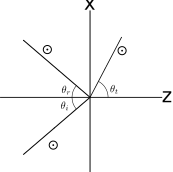
\includegraphics[width=.8\textwidth]{diagrams/RayGeometryDiagramS.eps}
\caption[Geometry for s polarization.]{Geometry for s polarization. Large arrows represent propagation direction of plane waves. Arrow tip indicators show that all electric fields point in the $+\mathbf{y}$ direction.
 \label{fig-rayGeometryDiagramS}}
\end{figure}

So far all results have assumed p polarization as depicted in figure \ref{fig-rayGeometryDiagramP}.  This section will investigate the slight changes that arise in the case of s polarization.  Because the math has already been worked out in detail once, and because the case of s polarization is somewhat simpler, the math shown here will be kept brief.

From the geometry depicted in figure \ref{fig-rayGeometryDiagramS}, it is clear that the wave vector expressions remain unchanged from equation \ref{eq-waveVectors}.  As a consequence, the spacial and temporal dependance in the electric fields do not change, and the law of reflection and Snell's law can be derived exactly as they were in section \ref{planeWaves-definitions}. Even the complex transmission angle, $\theta_t$, is defined exactly as it was for p polarization. However, the electric field expressions do change and it turns out they simplify considerably. The electric fields simplify so much that the boundary condition for the displacement field used to derive the reflection coefficient in the case of p polarized light is satisfied trivially and does not provide useful information to calculate the reflection coefficient. Instead the boundary conditions for tangential and normal magnetic fields suffice. As before, these conditions are also well established \cite{Jackson}. The system of equations analogous to equations \ref{eq-boundaryConditionsSubstitutedP} is similar.
\begin{subequations}
\begin{equation}\label{eq-boundaryConditionsSubstitutedS}
E_{0i}\cos\theta_i-E_{0r}\cos\theta_i=E_{0t}\cos\tilde{\theta_t}
\end{equation}
\begin{equation}
E_{0i}+E_{0r}=\frac{n_1}{\tilde{n}_2}E_{0t}
\end{equation}
\end{subequations}

After solving the system, it is clear that the amplitude reflection coefficient for s polarized light, denoted $\tilde{r}_s$, is similar to but simpler than the coefficient for p polarized light. In terms of refractive indices and known angles, $\tilde{r}_s$ can be expressed as,
\begin{equation}\label{eq-rs(n,theta)}
\tilde{r}_s=\frac{n_1\cos\theta_i-\tilde{n}_2\cos\tilde{\theta}_t}
{n_1\cos\theta_i+\tilde{n}_2\cos\tilde{\theta}_t}
\end{equation}
whereas, in terms of permittivities and wave vector components, it can be written
\begin{equation}\label{eq-rs(k,epsilon)}
\tilde{r}_s=\frac{k_{iz}-\tilde{k}_{tz}}{k_{iz}+\tilde{k}_{tz}}
\end{equation}

Because the wave vectors have already been calculated in the previous section, and discussion of their sign has been saved for the next section, the intensity reflection coefficient can be stated immediately.

\begin{equation}\label{eq-Rs}
R_s=\frac{(k_{iz}-k_{tz}')^2+k_{tz}''^2}{(k_{iz}+k_{tz}')^2+k_{tz}''^2}
\end{equation}

\section{Different Quadrants for $\tilde{k}_{tz}$}\label{planeWaves-differentQuadrants}

The final task is to determine an expression for the transmitted wave number's $z$-component, $\tilde{k}_{tz}$. Using $\tilde{k}_{tz}^2=\tilde{k}_t^2-k_{tx}^2$ with $\tilde{k}_t^2=(\epsilon_2'+i\epsilon_2'')k_0^2
=(n_2^2-\gamma^2-2in_2\gamma)k_0^2$, $\tilde{k}_{tz}^2$ can be expressed in terms of either refractive indices or permittivities as,
\begin{equation}\label{eq-ktz2Definition}
\tilde{k^2}_{tz}=k_0^2\left(n_2^2-\gamma^2-n_1^2\sin^2\theta_i-2in_2\gamma\right)
=k_0^2\left(\epsilon'_2-\epsilon_1\sin^2\theta_i+i\epsilon_2''\right)
\end{equation}
and $\tilde{k}_{tz}$ can then be evaluated as,
\begin{equation}\label{eq-ktzDefinition}
\tilde{k}_{tz}=\pm k_0\sqrt{n_2^2-\gamma^2-n_1^2\sin^2\theta_i-2in_2\gamma}
=\pm k_0\sqrt{\epsilon'_2-\epsilon_1\sin^2\theta_i+i\epsilon_2''}
\end{equation}

The fact that $\tilde{k}_{tz}$ is given by the  square root of equation \ref{eq-ktz2Definition} means that it will have two possible conjugate values.  This indeterminacy of $\tilde{k}_{tz}$ has led authors to draw very different conclusions about ATIR and the incidence angles at which it can exist. To proceed toward finding the solutions for $\tilde{k}_{tz}$'s real and imaginary parts, the real and imaginary parts of equation \ref{eq-ktz2Definition} can be equated to give a system of coupled equations in $k'_{tz}$, and $k''_{tz}$.
\begin{subequations}
\begin{equation}\label{eq-kSystemFirst}
k'^2_{tz}-k''^2_{tz}=k_0^2(n_2^2-\gamma^2-n_1^2\sin^2\theta_i)
\end{equation}
\begin{equation}\label{eq-signControl}
k'_{tz}k''_{tz}=-k_0^2n_2\gamma
\end{equation}
\end{subequations}

Solving \ref{eq-signControl} first for $k'_{tz}$, then for $k''_{tz}$, and substituting into \ref{eq-kSystemFirst} yields the following decoupled quadratics for $k'^2_{tz}$ and $k''^2_{tz}$.
\begin{equation}\label{eq-ktzSystem}
\left.
\begin{aligned}
k'^4_{tz}  - [n_2^2-\gamma^2-n_1^2\sin^2\theta_i]k_0^2k'^2_{tz}  - k_0^4n_2^2\gamma^2 = 0 \\
k''^4_{tz} + [n_2^2-\gamma^2-n_1^2\sin^2\theta_i]k_0^2k''^2_{tz} - k_0^4n_2^2\gamma^2 = 0
\end{aligned}
\right\}
\end{equation}
or
\begin{equation}\label{eq-ktzSystemEpsilon}
\tag{\ref{eq-ktzSystem}'}
\left.
\begin{aligned}
k'^4_{tz}  - [\epsilon_2'-\epsilon_1\sin^2\theta_i]k_0^2k'^2_{tz}  - \frac{k_0^4\epsilon_2''^2}{4} = 0 \\
k''^4_{tz} + [\epsilon_2'-\epsilon_1\sin^2\theta_i]k_0^2k''^2_{tz} - \frac{k_0^4\epsilon_2''^2}{4} = 0
\end{aligned}
\right\}
\end{equation}
Because the gain parameters, $\gamma$ and $\epsilon_2''$, appear squared in equations \ref{eq-ktzSystem}, both $k'_{tz}$ and $k''_{tz}$ have the same magnitudes regardless of whether the second medium is gainy or lossy. The fact that equations (\ref{eq-ktzSystem}) are quartic suggests that there may be four solutions for $\tilde{k}'_{tz}$ and another four solutions for $\tilde{k}''_{tz}$ given as follows.

\begin{equation}
k'_{tz}=\pm \frac{k_0}{\sqrt{2}}\sqrt{\epsilon'_2-\epsilon_1\sin^2\theta_i \pm \sqrt{(\epsilon'_2-\epsilon_1\sin^2\theta_i)^2+\epsilon''^2_2}}
\end{equation}
\begin{equation}
k''_{tz}=\pm \frac{k_0}{\sqrt{2}}\sqrt{\epsilon_1\sin^2\theta_i-\epsilon'_2 \pm \sqrt{(\epsilon'_2-\epsilon_1\sin^2\theta_i)^2+\epsilon''^2_2}}
\end{equation}
However, $k'_{tz}$ and $k''_{tz}$ were defined in equation \ref{eq-kPrimesDefinition} to be strictly real. Consequently, the signs preceding the inner square roots above must both be positive, reducing the preceding equations to,

\begin{equation}\label{eq-ktz'Solution}
k'_{tz}=\pm \frac{k_0}{\sqrt{2}}\sqrt{\epsilon'_2-\epsilon_1\sin^2\theta_i+\sqrt{(\epsilon'_2-\epsilon_1\sin^2\theta_i)^2+\epsilon''^2_2}}
\end{equation}
\begin{equation}\label{eq-ktz''Solution}
k''_{tz}=\pm \frac{k_0}{\sqrt{2}}\sqrt{\epsilon_1\sin^2\theta_i-\epsilon'_2+\sqrt{(\epsilon'_2-\epsilon_1\sin^2\theta_i)^2+\epsilon''^2_2}}
\end{equation}

Equation \ref{eq-signControl} dictates that the real and imaginary parts of $\tilde{k}_{tz}$ must have opposite signs for $\gamma > 0$ (gainy second medium) and the same sign for $\gamma < 0$ (lossy second medium). This restricts the complex quantity $\tilde{k}_{tz}$ to lie in either the second or fourth quadrant in the case of a gainy second medium, and the first or third quadrant in the case of a lossy second medium. So $\tilde{k}_{tz}$ has indeed been reduced to two possible solutions as was expected initially from equation \ref{eq-ktzDefinition}.

The ultimate question that needs to be answered is which of the two mathematically valid solutions for $p_{tz}$ is physically correct in each of the four cases where the incidence is below or above the critical angle on a lossy or gainy medium. To answer the question, we must first observe that the $z$-dependent phase factor in the plane wave is given by
\begin{equation}\label{eq-phaseFactor}
e^{i\tilde{k}_{tz}z}=e^{ik_{tz}'z-k_{tz}''z}
\end{equation}

The physically correct solution is defined by the following three conditions.
\begin{enumerate}\label{conditions}
\item A wave's amplitude must grow in the propagation direction in a gainy medium and decay in a lossy medium.
\item The solution corresponding to a non-evanescent wave behind the boundary, when $\theta_i < \theta_c$ and $|k_{tz}''| \ll k_{tz}'$, must propagate away from the boundary in either lossy or gainy media.
\item The solution corresponding to an evanescent wave behind the boundary, when $\theta_i > \theta_c$ and $|k_{tz}''| \gg k_{tz}'$, must decay away from the boundary in either lossy or gainy media.
\end{enumerate}

\begin{figure}[htb]
\centering
  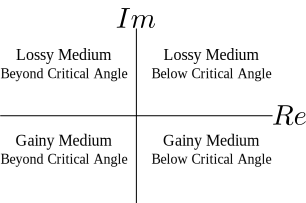
\includegraphics[width=.6\linewidth]{diagrams/fig-ComplexPlaneSummary.eps}
\caption[Complex plane diagram for $\tilde{k}_{tz}^2$]{$\tilde{k}_{tz}^2$ will lie in different quadrants depending on the gain factor's sign and the incident angle.
 \label{fig-complexPlaneSummary}}
\end{figure}

Figure \ref{fig-complexPlaneSummary} summarizes the conditions under which $\tilde{k}^2_{tz}$ lies in various quadrants of the complex plane. In the next sections, each of the four cases will be discussed, and the proper root, $\tilde{k}_{tz}$, will be chosen.


\subsection{Lossy Medium Below Critical Angle}

\begin{figure}[ht]
\centering
  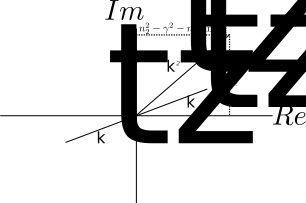
\includegraphics[width=\linewidth]{diagrams/fig-ComplexPlaneQ1.eps}
\caption[$\tilde{k}_{tz}^2$ complex plane diagram, $\gamma<0$, $\theta_i<\theta_c$]{For lossy second medium and incidence below the critical angle, $\tilde{k}_{tz}^2$ lies in the first quadrant. It's conjugate roots lie in the first and third quadrants.
 \label{fig-complexQ1}}
\end{figure}

We will begin by investigating the case of a lossy second medium because the solution is not debated, and it will serve as an introduction to the case of a gainy second medium, which is widely debated.  When the incident angle is below the critical angle, the quantity $\tilde{k}_{tz}^2$ lies in the first quadrant as illustrated in figure \ref{fig-complexQ1}. The two mathematical solutions for $\tilde{k}_{tz}$ in this case lie in the first and third quadrants.

The imaginary part of $\tilde{k}^2_{tz}$ is determined only by properties of the media, whereas the real part depends on incident angle as well. As the incident angle increases from normal incidence up to the critical angle, the location of $\tilde{k}^2_{tz}$ in the complex plane traces a horizontal line to the left such that it lies along the positive imaginary axis at the critical angle.

\begin{figure}[ht]
\centering
  \includegraphics[width=\linewidth]{plots/fig-LossyReflectivitiesOptionsBelowCriticalAngle.eps}
\caption[Two possible Reflectivities from lossy medium below critical angle]{The two curves depict the possible reflectivities, $R$ from the lossy medium at incidence below the critical angle. Only the curve below unity is physically correct. 
 \label{fig-LossyReflectivitiesOptionsBelowCriticalAngle}}
\end{figure}

Choosing the correct physical solution for $\tilde{k}_{tz}$, will dictate whether the reflected wave is amplified or attenuated. The two possible reflectivities, calculated from equation \ref{eq-R}, are plotted in figure \ref{fig-LossyReflectivitiesOptionsBelowCriticalAngle}. The $z$-dependent phase factor from equation \ref{eq-phaseFactor} can be written with all signs explicitly shown as,

\begin{equation}
e^{i\tilde{k}_{tz}} = \begin{cases}
    e^{i|k'_{tz}|z-|k''_{tz}|z}       & 1^{st} Quadrant \\
    e^{-i|k'_{tz}|z+|k''_{tz}|z}      & 3^{rd} Quadrant
\end{cases}
\end{equation}
so that the three previously stated conditions can be more easily used to determine the quadrant of $\tilde{k}_{tz}$. Condition one requires that the wave's amplitude decay in its propagation direction. The Q1 solution is right-traveling, and decaying as $z$ increases, so it satisfies the first condition. The Q3 solution is left-traveling and decaying as $z$ decreases, so it also satisfies the first condition.  Because this wave is incident below the critical angle, it is not evanescent and  condition two requires that it travel away from the boundary, in the $+z$ direction. The sign in front of $|k''_{tz}|$ above indicates that only the Q1 solution meets this requirement, so we can conclude that it is the physically correct solution.

\subsection{Lossy Medium Beyond Critical Angle}
When the incidence angle increases beyond the critical angle, $\tilde{k}_{tz}^2$ moves from the first quadrant into the second following the same horizontal line that it did previously.  The two conjugate roots remain in the first and third quadrants.

\begin{figure}[ht]
\centering
  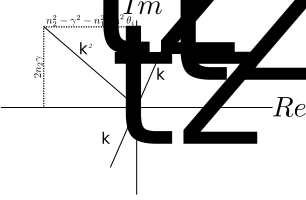
\includegraphics[width=\linewidth]{diagrams/fig-ComplexPlaneQ2.eps}
\caption[$\tilde{k}_{tz}^2$ complex plane diagram, $\gamma<0$, $\theta_i>\theta_c$]{For lossy second medium and incident angle beyond the critical angle, $\tilde{k}_{tz}^2$ lies in the second quadrant. It's conjugate roots remain in the first and third quadrants.
 \label{fig-complexQ2}}
\end{figure}

As before, the $z$-dependent phase factor from equation \ref{eq-phaseFactor}, written with all signs explicitly shown, is

\begin{equation}
e^{i\tilde{k}_{tz}} = \begin{cases}
    e^{i|k'_{tz}|z-|k''_{tz}|z}       & 1^{st} Quadrant \\
    e^{-i|k'_{tz}|z+|k''_{tz}|z}      & 3^{rd} Quadrant
\end{cases}
\end{equation}

\begin{figure}[ht]
\centering
  \includegraphics[width=.8\linewidth]{plots/fig-LossyReflectivitiesOptionsBeyondCriticalAngle.eps}
\caption[Two possible Reflectivities from lossy medium above critical angle]{The two curves depict the possible reflectivities, $R$ from the lossy medium at incidence beyond the critical angle. Only the curve below unity is physically correct.
 \label{fig-LossyReflectivitiesOptionsBeyondCriticalAngle}}
\end{figure}

The two resulting reflectivity options from equation \ref{eq-R} are shown in figure \ref{fig-LossyReflectivitiesOptionsBeyondCriticalAngle}.

The first of the conditions on page \pageref{conditions} is satisfied by both solutions as it was for incidence below the critical angle. However, the second condition, which determined the physically correct solution for incidence below the critical angle, no longer applies because the wave in medium two has become evanescent. Rather the third condition requires that the evanescent wave decays away from the boundary. The positive sign in front of $|k''_{tz}|$ makes it clear that the Q3 solution will grow exponentially in medium two, leaving the Q1 solution, which decays away from the boundary, as the physically correct solution.

\begin{figure}[ht]
\centering
  \includegraphics[width=.9\linewidth]{plots/fig-Q1ReflectivityP.eps}
\caption[Reflectivity, $R$, from lossy medium at various losses.]{First quadrant reflectivity, $R$, from lossy second medium plotted for various values of loss. Notice that for any nonzero loss, the reflectivity does not reach zero at the Brewster angle.\label{fig-Q1ReflectivityP}} 
\end{figure}

In addition to meeting the requirements outlined for the physically correct solution, the Q1 solution provides attenuated TIR  both below and beyond the critical angle. The Q3 solution would provide amplified TIR violating energy conservation. This is further assurance that satisfying the three conditions has led to the physically correct solution.

Having chosen the Q1 solution for a lossy second medium both below and beyond the critical angle, the complete reflectivity curves are plotted for various values of loss in figure \ref{fig-Q1ReflectivityP}

\subsection{Gainy Medium Below Critical Angle}
Having resolved the lossy second medium case, we can now discuss the debated case of a gainy second medium. When a wave is incident below the critical angle on a gainy second medium, $\tilde{k}_{tz}^2$ lies in the fourth quadrant and the conjugate roots, have now shifted from the first and third quadrants to the second and fourth as depicted in figure \ref{fig-complexQ4}. As in the case of a lossy second medium, as the incident angle increases from the normal to the critical angle,  $\tilde{k}_{tz}^2$ moves horizontally to the left until it is resting on the negative imaginary axis.

\begin{figure}[htb]
\centering
  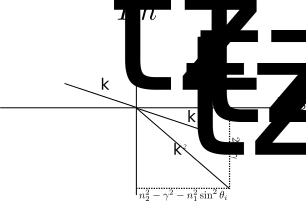
\includegraphics[width=\linewidth]{diagrams/fig-ComplexPlaneQ4.eps}
\caption[$\tilde{k}_{tz}^2$ complex plane diagram, $\gamma>0$, $\theta_i<\theta_c$]{For gainy second medium and incident angle below the critical angle, $\tilde{k}_{tz}^2$ lies in the fourth quadrant. It's conjugate roots lie in the fourth and second quadrants.
 \label{fig-complexQ4}} 
\end{figure}

The  plane wave reflectivity options from equation \ref{eq-R}, resulting from the new quadrants for $\tilde{k}_{tz}$, are plotted in figure \ref{fig-GainyReflectivitiesOptionsBelowCriticalAngle}. The curves are the same as figure \ref{fig-LossyReflectivitiesOptionsBelowCriticalAngle} in the lossy case, although the quadrant for $\tilde{k}_{tz}$ is importantly not. This illustrates the important general rule that reflectivities will be the same for conjugate loss and gain media if the corresponding quadrants for $\tilde{k}_{tz}$ are chosen. This is a consequence of the fact that the gain factor, $\gamma$ appears squared in equations \ref{eq-ktzSystem}.

\begin{figure}[htb]
\centering
  \includegraphics[width=\linewidth]{plots/fig-GainyReflectivitiesOptionsBelowCriticalAngle.eps}
\caption[Two possible Reflectivities from gainy medium below critical angle]{The two curves depict the possible reflectivities, $R$ from a gainy medium at incidence below the critical angle. Only the curve below unity is physically correct.\label{fig-GainyReflectivitiesOptionsBelowCriticalAngle}} 
\end{figure}

In the literature, authors are not unanimously agreed on the physically correct quadrant for $\tilde{k}_{tz}$ in this case as they are in the case of lossy media. Most authors, including \cite{Romanov} \cite{Fan} \cite{Willis} and \cite{Mansuripur}, have chosen the fourth quadrant solution leading to attenuated reflection below the critical angle, whereas the authors of \cite{CandC} have chosen the second quadrant solution leading to Amplified TIR. As usual, the physically correct solution can be discerned by writing the $z$ dependent phase factor from equation \ref{eq-phaseFactor}. Unlike the lossy case, equation, \ref{eq-signControl} requires that real and imaginary parts of $\tilde{k}_{tz}$ have the same sign in the gainy case.

\begin{equation}
e^{i\tilde{k}_{tz}} = \begin{cases}
    e^{-i|k'_{tz}|z-|k''_{tz}|z}       & 2^{nd} Quadrant \\
    e^{i|k'_{tz}|z+|k''_{tz}|z}        & 4^{th} Quadrant
\end{cases}
\end{equation}

The second quadrant solution is left-traveling and its amplitude grows at it travels, whereas the fourth quadrant solution is right-traveling and also growing as it travels. So the first condition is again satisfied for both solutions. Because the transmitted wave is non-evanescent, condition two requires that it propagate away from the boundary. The fourth quadrant solution satisfies this condition, but the left-traveling second quadrant solution does not. The fourth quadrant solution is the only physically correct solution. It is not useful to plot the solution at various gains because the curves would be identical to those of the conjugate loss medium in figure \ref{fig-Q1ReflectivityP} below the critical angle.

Callary and Carniglia, the authors of \cite{CandC}, were led to support the existence of the second quadrant solution in this case because they began by analyzing the three layer problem -- two transparent media with a gainy slab between them. They concluded that waves corresponding to both the Q2 and the Q4 solutions would exist in the slab because reflection from the third layer, would convert one solution to the other. Using their three layer results in the limit as $d\to\infty$, they concluded that amplified reflection was possible from a single surface. Their mistake derived from the fact that in the true two layer problem, there is no back surface from which a wave can reflect. The authors viewed their result as a theoretical explanation of the gain of 1000 observed by the Kogan et. al. experiment \cite{Kogan2}. But while their theory did explain the high gain observed experimentally, the experimental result was a consequence of the three layer configuration that they treated rather than a strictly single surface phenomenon.

\subsection{Gainy Medium Beyond Critical Angle}

\begin{figure}[htb]
\centering
  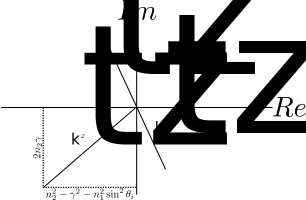
\includegraphics[width=\linewidth]{diagrams/fig-ComplexPlaneQ3.eps}
\caption[$\tilde{k}_{tz}^2$ complex plane diagram, $\gamma>0$, $\theta_i>\theta_c$]{For gainy second medium and incident angle beyond the critical angle, $\tilde{k}_{tz}^2$ lies in the third quadrant. It's conjugate roots remain in the fourth and second quadrants. 
 \label{fig-complexQ3}}
\end{figure}
The final case that remains to be analyzed is incidence beyond the critical angle on a gainy second medium. Under these conditions, the incidence angle has become great enough that $\tilde{k}^2_{tz}$ has moved into the third quadrant. The possible conjugate roots remain in the second and fourth quadrants as they were for incidence below the critical angle.

In this case, the $z$ dependent phase factor can be written as it was in the previous section.

\begin{equation}
e^{i\tilde{k}_{tz}} = \begin{cases}
    e^{-i|k'_{tz}|z-|k''_{tz}|z}       & 2^{nd} Quadrant \\
    e^{i|k'_{tz}|z+|k''_{tz}|z}        & 4^{th} Quadrant
\end{cases}
\end{equation}

It has already been stated that the first of the three conditions is satisfied by both solutions. Beyond the critical angle, the transmitted wave is evanescent, so the third condition requires that its amplitude decay away from the boundary. The negative sign in front $|k''_{tz}|z$ in the Q2 solution indicates that it meets this requirement, while the positive sign in front of $|k''_{tz}|z$ in the Q4 solution indicates an exponentially growing wave.  This leaves Q2 as the only physically correct solution.

The two possible options have not been plotted beyond the critical angle because they are, again, identical to those in figure \ref{fig-LossyReflectivitiesOptionsBeyondCriticalAngle}. The reflectivities are shown at all incident angles in figures \ref{fig-gainyReflectivityFinal-lowGain} and \ref{fig-gainyReflectivityFinal-highGain} for various values of the gain factor, $\gamma$.

\begin{figure}[htb]
\centering
\includegraphics[width=\textwidth]{plots/fig-gainyReflectivityFinal-lowGain.eps}
\caption[Final Reflectivity for Plane Waves -- Low Gain]{Surface reflectivity $R$ for plane waves on a gainy second medium. Reflectivity is discontinuous at the critical angle where $k_{tz}$ switches from the fourth quadrant to the second.
 \label{fig-gainyReflectivityFinal-lowGain}}
\end{figure}

\begin{figure}[htb]
\centering
\includegraphics[width=\textwidth]{plots/fig-gainyReflectivityFinal-highGain.eps}
\caption[Final Reflectivity for Plane Waves -- High Gain]{Surface reflectivity $R$ for plane waves on a gainy second medium. With higher gain present it becomes clear that there is a maximum reflectivity for given $n_1$ and $n_2$. It also becomes clear that the critical angle moves closer to the normal as gain increases.
 \label{fig-gainyReflectivityFinal-highGain}}
\end{figure}


The Mansuripurs, the authors of \cite{Mansuripur}, argue that the second quadrant solution is ``unlikely" on the grounds that as the incidence angle increases from just below the critical angle to just above it, $\tilde{k}_{tz}$ jumps discontinuously from the fourth quadrant to the second quadrant. Because no such discontinuous jump exists in the case of classical TIR from transparent media, where $\tilde{k}_{tz}$ is strictly real below the critical angle, zero at that angle, and strictly imaginary above it, the authors argue that no discontinuity need exist for gainy media either. Their argument is incorrect for two reasons. First, the case of TIR from transparent media is a special case of that which is presently being treated in which $\tilde{k}_{tz}$ does not jump discontinuously at the critical angle only because the Q4 and Q2 solutions are degenerate, both being equal to zero. Second, in the case of lossy or gainy media, a discontinuity in $\tilde{k}_{tz}$ \textit{must} exist under some conditions. Choosing the Q2 solution eliminates the discontinuity at the critical angle, but creates one when a wave is incident beyond the critical angle and the second media is tuned from gainy to lossy. This is illustrated in the summarizing diagram in the next section.



\subsection{Conclusions and Experimental Evidence}
Based on the arguments in the previous sections, I choose the first quadrant solution for $\tilde{k}_{tz}$ at all incidence angles if the second medium is lossy. But, if the second medium is gainy, the fourth quadrant solution is chosen only below the critical angle, while the second quadrant solution takes over beyond $\theta_c$, resulting in ATIR, beyond the critical angle.

\begin{figure}[htb]
\centering
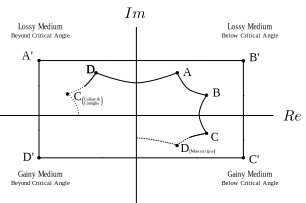
\includegraphics[width=\textwidth]{diagrams/fig-ComplexPlaneSummaryDetailed.eps}
\caption[Detailed quadrant summary of $\tilde{k}^2_{tz}$ and $\tilde{k}_{tz}$ under various conditions]{Detailed quadrant summary of $\tilde{k}^2_{tz}$ (rectangle) and $\tilde{k}_{tz}$ (solid inner locus) under various conditions. Dotted line indicates Callary and Carniglia's alternate locus. Dashed line indicates Mansuripurs' alternate locus. No theory suggests a locus in the third quadrant -- it would mean ATIR from lossy media.
 \label{fig-ComplexPlaneSummaryDetailed}}
\end{figure}

Figure \ref{fig-ComplexPlaneSummaryDetailed} summarizes this information in the context of a hypothetical experiment. Imagine a lab setup such that both incident angle and second media gain/loss were controlled by knobs. The system is initially configured such that $\tilde{k}_{tz}^2$ lies at point $A'$ corresponding to an incident wave striking a lossy medium at a glancing angle with $\tilde{k}_{tz}$ at point $A$ on the inner locus.  As the incidence angle is tuned from glancing, through the critical angle, down to near normal incidence, $\tilde{k}^2_{tz}$ and $\tilde{k}_{tz}$ advance to points $B'$ and $B$. Maintaining near normal incidence, $\gamma$ is increased, from lossy, through transparent, to gainy, and $\tilde{k}^2_{tz}$ and $\tilde{k}_{tz}$ reach points $C'$ and $C$. Callary and Carniglia disagree about the location of point $C$, and claim that $\tilde{k}_{tz}$ experiences a discontinuous jump to the second quadrant as the medium becomes transparent which is indicated with a dotted line. With the second medium now gainy, the incidence angle is again tuned through the critical angle, back to glancing incidence, and the loci advance to points $D$ and $D'$. This time it is the Mansuripurs who disagree about the location of point $D$, and their alternate locus is indicated with a dashed line. Finally $\gamma$ is tuned back to lossy and the loci return to points $A$ and $A'$.

The theory and quadrant choices outlined in this section are able to explain all experimental data to date. The Koester fiber experiment deals with multiple reflections, beyond the critical angle, so even a small gain on each reflection could account for his results. The gain of 25 observed by Kogan et.al. is feasible from single surface ATIR, and can also be explained according to the three layer theory of Callary and Carniglia. The gain of 1000 observed by Kogan et. al. could only be explained by single surface ATIR if the second quadrant were chosen for incidence angles below the critical angle, which I have argued to be physically incorrect. Rather their exceedingly high gain must be explained in terms of a third layer according to the theory of Callary and Carniglia.

%XXXXXXXXXXXXXXXXXXXXXXXXXXXXXXXXXXXXXXXXXXXXXXXXXXXXXXXXXXXXXXXXXXXX

\chapter{Case of a Finite Beam}\label{chap-finiteBeam}
As was mentioned in section \ref{intro-TIR}, a real world light beam is never a true plane wave. In order to make meaningful predictions about experimental results, I will now treat the case of a finite width beam. The exact profile of the beam is not critically important; any finite beam will do. It is customary in the literature \cite{Konopsky}\cite{Willis} to treat a Gaussian profile, and I will do likewise. The Gaussian profile is very convenient because it closely approximates the true profile of a laser beam produced from a cavity in its TEM${}_{0,0}$ mode.

Until now, all results have been analytical and exact. The formulas derived for plane wave reflection in equations \ref{eq-r(k,epsilon)}, \ref{eq-R}, \ref{eq-rs(k,epsilon)}, and \ref{eq-Rs} were in closed form without approximation.  In this chapter approximations and numerical work will be necessary to treat the additional mathematical complexity of finite beams and Fourier analyses. I will discuss and use methods to minimize error throughout the chapter, but ultimately approximate results will still be quite useful as the main intention is to gain understanding of how finite beams differ from plane waves, not to exactly solve for the reflectivity of a particular finite beam profile.

\section{Derivation and Properties of a Gaussian Beam}
The derivation of a Gaussian beam is well established, and found in many text books (eg. \cite{Boyd}), so it will be outlined here only briefly. Attention rather will be placed on the properties and parameters of the beam.

It is convenient to define a set of primed coordinates that are the beam's natural coordinates, such that the beam travels primarily along the $z'$ direction. Starting from the Helmholtz wave equation,
\begin{equation}\label{eq-helmholtz}
\nabla^2\tilde{A}+k^2\tilde{A}=0\,,
\end{equation}
if the cross-sectional profile of the beam changes slowly as the beam propagates, the so-called paraxial approximation, $\partial A/\partial z \ll kA$, can be made to reduce equation \ref{eq-helmholtz} to its paraxial form.

\begin{equation}\label{eq-paraxial}
\frac{\partial\tilde{A}}{\partial x^2}+\frac{\partial\tilde{A}}{\partial y^2}+2ik\frac{\partial A}{\partial z} =0
\end{equation}

\begin{figure}[htb]
\centering
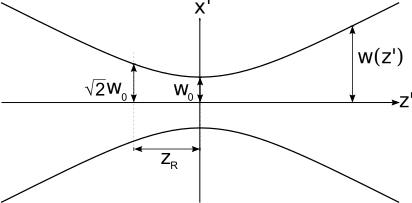
\includegraphics[width=.9\textwidth]{diagrams/fig-gaussianParameters.eps}
\caption[Gaussian beam diagram showing beam waist and Rayleigh range]{Width of a Gaussian beam near its waist (at $z'=0$). Rayleigh range and beam width are shown.
 \label{fig-gaussianParameters}}
\end{figure}

In the case of a wave traveling in the $z'$ direction the complex electric field amplitude is given by $E(\mathbf{x'})=\tilde{A}(\mathbf{x'})e^{ikz'}$, and the field of a Gaussian beam  satisfying the paraxial wave equation, has the general form,

\begin{equation}\label{eq-gaussian}
E(\mathbf{x'})=E_0\frac{w_0}{w^2(z')}\exp\left[
-\frac{x'^2+y'^2}{w^2(z')}+ik\left(z'-\frac{x'^2+y'^2}{2R(z')}\right)+i\xi(z')
\right]
\end{equation}
where it remains to define the quantities $w(z')$, $R(z')$, and $\xi(z')$.

\begin{figure}[htb]
\centering
\includegraphics[width=.9\textwidth]{plots/fig-gaussianProfilesVariousZ.eps}
\caption[Cross-section intensity profiles of a Gaussian beam.]{Cross-section intensity profiles of a Gaussian beam at various longitudinal positions. The cross section is always Gaussian, its radius is not constant.
 \label{fig-gaussianProfilesVariousZ}}
\end{figure}

The cross-sectional intensity profile of the beam described in equation \ref{eq-gaussian} is Gaussian at any point as seen in figure \ref{fig-gaussianProfilesVariousZ}, but its radius is not constant. The beam reaches a narrowest point, $w_0=w(0)$, known as its waist, at $z'=0$.  In the paraxial approximation, plane waves must travel primarily in the beam's propagation direction. In order to keep this approximation valid, the beam cannot be focused more narrowly than about one wavelength, $w_0>\lambda$. The beam width at any point other than $z=0$ is defined as the radius at which the electric field amplitude falls to $(1/e)$-th of its value on the central axis. This is illustrated in figure \ref{fig-gaussianParameters} and given functionally as follows.
\begin{equation}\label{eq-beamWidth}
w(z)=w_0\sqrt{1+\left(\frac{z'}{z_R}\right)^2}
\end{equation}

The additional longitudinal distance, $z_R$, is referred to as the Rayleigh range and defined as the propagation distance at which the beam waist has increased by a factor of $\sqrt{2}$, also illustrated in figure \ref{fig-gaussianParameters}.
\begin{equation}\label{eq-rayleighRange}
z_R=\frac{\pi w_0^2}{\lambda}=\frac{w_0^2k}{2}
\end{equation}

The surfaces of constant phase in the beam make spherical wave fronts which are described in terms of their radius, $R(z')$. It is important that $R$ is not measured from the primed coordinate origin to a phase front, but rather from the center of the phase front's arc to the phase front itself as illustrated in figure \ref{fig-gaussianRadius}.
\begin{equation}\label{eq-curvatureRadius}
R(z')=z'\left(1+\left(\frac{z_R}{z'}\right)^2\right)
\end{equation}

\begin{figure}[htb]
\centering
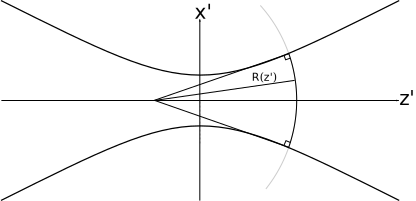
\includegraphics[width=.9\textwidth]{diagrams/fig-gaussianRadius.eps}
\caption[Gaussian beam diagram showing phase front radius]{Gaussian beam near its waist. Phase front curvature, $R(z')$ is shown. Note: $R(z')$ is not measured from the coordinate origin.
 \label{fig-gaussianRadius}}
\end{figure}

Because the Gaussian beam is composed of many plane waves traveling in slightly different directions, it's phase behaves in an unusual way. First of all the phase is not constant in $x'$ (or $y'$) for fixed $z'$. Second, the beam goes through an additional phase shift of $\pi$ radians near its waist which is described by the Gouy phase, $\xi(z')$, given as follows.

\begin{equation}\label{eq-gouy}
\xi(z')=\arctan(z'/z_R)
\end{equation}



\subsection{Coordinate Systems for Reflection}

\begin{figure}[ht]
\centering
\begin{minipage}{.5\textwidth}
  \includegraphics[width=\linewidth]{diagrams/fig-gaussianAxesIncident.eps}
\end{minipage}%
\begin{minipage}{.5\textwidth}
  \includegraphics[width=\linewidth]{diagrams/fig-gaussianAxesReflected.eps}
\end{minipage}
\caption[Natural axes of incident and reflected Gaussian beams]{Natural axes of incident (left, primed) and reflected (right, doubly primed) Gaussian Beams. $z'$ and $z''$ axes are the primary propagation directions. Curved lines show the beam width along the propagation directions.
  \label{fig-gaussianAxes}}
\end{figure}

The Gaussian beam is expressed most naturally and easily in its natural coordinate system. It will therefore be necessary to relate the natural coordinates of the incident and reflected beams to the surface coordinates used until now. The Gaussian beam's central ray strikes the surface at angle $\phi$. This nomenclature is chosen to distinguish the special central ray from the constituent plane waves in the rest of this chapter. Figure \ref{fig-gaussianAxes} shows the three coordinate systems as well as the beam widths for the incident and reflected beams. Note that all of the coordinate systems are simply related to one another by rotations through the incidence (and reflection) angle, $\phi$. In particular, transformations between the three sets of axes can be easily accomplished using the following relations.
\begin{subequations}\label{eq-primedTransform}
\begin{equation}
z'=z\cos\phi+x\sin\phi \qquad 
x'=x\cos\phi-z\sin\phi
\end{equation}
\begin{equation}
x=x'\cos\phi+z'\sin\phi \qquad
z=z'\cos\phi-x'\sin\phi
\end{equation}
\end{subequations}

\begin{subequations}\label{eq-doublePrimedTransform}
\begin{equation}
z''=-z\cos\phi_i+x\sin\phi \qquad 
x''=-x\cos\phi-z\sin\phi
\end{equation}
\begin{equation}
x=-x''\cos\phi+z''\sin\phi \qquad
z=-z''\cos\phi-x''\sin\phi
\end{equation}
\end{subequations}

\section{Fourier Analysis of Finite Beams}
Having thoroughly treated the case of incident plane waves in the previous chapter, the behavior of a finite width beam can be understood by expressing it as a superposition of constituent plane waves. This is accomplished through use of the Fourier transform, which expresses the wave's electric field as a function of parallel wave number components, $k_{ix}$, or plane wave incident angles, $\theta_i$. That is, the Fourier transform describes how much of the finite beam's intensity is present in each of the constituent plane waves that travel in slightly different directions. For this treatment, it will not be necessary to consider the direction perpendicular to the incidence plane (the $y$-direction), so this coordinate will be suppressed for the remainder of the chapter, and electric fields will be written as functions of $x$ and $z$ only.

To begin, the beam must be written in terms of its natural coordinate system as in equation \ref{eq-gaussian}. The transform can be computed at any location, and in any of the three coordinate systems to provide information about the intensity contained in each plane wave. But in order to get the correct reflection from the surface, the phase information, and consequently the complex electric field, must be known at the surface. Therefore, it is necessary to use the coordinate system transformation equations \ref{eq-primedTransform} to write the incident electric field in terms of unprimed coordinates.

\begin{equation}
\left. E_i(x', z') \right|_{z=0}(x) = E_i(x\cos\phi, x\sin\phi)
\end{equation}

In particular,
\begin{equation}\label{eq-gaussianSurface}
\begin{aligned}
&E_i(x) \approx \frac{E_0}{\sqrt{1+\frac{x^2\sin^2\phi}{z_R^2}}} \\
 &\exp\left[
  \frac{-x^2\cos^2\phi}{w_0^2\left(1+\frac{x^2\sin^2\phi}{z_R^2}\right)}
  +ikx\sin\phi
  -ik\frac{x\cos^2\phi}{2\sin\phi\left(1+\frac{z_R^2}{x^2\sin^2\phi}\right)}
  +i\arctan\left(\frac{x\sin\phi}{z_R}\right)
\right]
\end{aligned}
\end{equation}

Using the surface expression for the incident electric field, the Fourier transform can be taken to give the necessary amplitude and phase information at the surface.

\begin{equation}\label{eq-fourierTransform}
E_i(k_x)=\int_{-\infty}^\infty E_i(x) e^{-ik_xx}\,\mathrm{d}x
\end{equation}

With the incident beam now decomposed into constituent plane waves, each plane wave can be reflected from the surface according to the theory of chapter \ref{chap-planeWaves} using equation \ref{eq-r(k,epsilon)} for $p$-polarization or equation \ref{eq-rs(k,epsilon)} for $s$-polarization.

\begin{equation}
E_r(k_x) = E_i(k_x) \tilde{r}(k_x)\,.
\end{equation}
The reflected beam can then be reconstructed by integrating over all reflected plane waves. Note that the kernel of the inverse transform can include an additional $z$ dependent term used to propagate the beam away from the reflection surface, with the $z$-component wave numbers calculated as $k_z = \sqrt{k^2-k_x^2}$. Or, alternatively, the transform can be written in terms of plane wave incidence angles rather than wave vector components.

\begin{equation}\label{eq-inverse-transform}
E_r(x, z) = \int_{-\infty}^\infty E_r(k_x)e^{i(k_xx+k_zz)}\,\mathrm{d}k_x
= \int_{-\pi/2}^{\pi/2} E_r(\theta_i)e^{ik(\sin\theta_ix+\cos\theta_iz)}\,\mathrm{d}\theta_i\,.
\end{equation}

If it is necessary or convenient, the reflected beam can be transformed into its own natural coordinates, the doubly primed coordinates, by use of equations \ref{eq-doublePrimedTransform}.

In the next two sections, the steps outlined here will be performed in detail both analytically and numerically and the differences between the two methods will be discussed.

\subsection{Analytical Method with Approximations}
The expression for the incident field at the reflecting surface given in equation \ref{eq-gaussianSurface} is as exact as the expression in equation \ref{eq-gaussian}. The only approximation so far is that it is a solution to the paraxial form of the Helmholtz equation. Consequently, the only limitation to keep in mind is that the spot size must be larger than about one wavelength. However, the expression for $E_i(x)$ on the surface is too complex to be transformed analytically according to the integral in equation \ref{eq-fourierTransform}, so two more approximations will be necessary.

The first issue to consider is the arctan term that arises from the Gouy phase. Using a small angle approximation, this term can be simplified to $\arctan\left(\frac{z'}{z_R}\right) \approx \frac{z'}{z_R}$, which leaves off all terms in the Taylor series expansion of $\mathcal{O}(z'^3)$ and higher. The approximation is quite good when the beam strikes the surface near normal incidence, but becomes arbitrarily bad as the incidence angle, $\phi$, increases. Alternately a large angle approximation allows the simplification $\arctan\left(\frac{z'}{z_R}\right) \approx \frac{\pi}{2}-\frac{z_R}{z'}$, which leaves off all terms of $\mathcal{O}(z'^{-3})$. Again, this approximation is good at glancing incidence, but arbitrarily bad near normal incidence. Because we want to treat the full domain of incidence angles, and because the true arctan never exceeds $\pm\pi/2$, it is a good approximation to neglect the Gouy phase entirely.
\begin{equation}
\arctan\left(\frac{z'}{z_R}\right) \approx 0
\end{equation}
This approximation simplifies the integration considerably, and introduces less error over the full range of incidence than either of the previously mentioned alternatives.  If a higher degree of accuracy is desired for a particular incidence angle, the Taylor series expansion can be performed around that point. As we will see, a first order expansion never increases the difficulty of analytical integration.

Removing the Gouy phase from the exponential is helpful, but further simplification will be necessary to perform the Fourier transform analytically. The second approximation is to assume that the beam focus remains wide enough that for all values of $x$ on the surface, within the beam's width,
\begin{equation}\label{eq-approximation}
x^2/z_R^2 \ll 1\,,
\end{equation}
which reduces the beam width to the constant $w_0$, and allows the $1$ term in the curvature radius to be neglected leaving $R(z')\approx z_R^2/z'$. The approximation can then be applied again, eliminating this term entirely because it is small compared to the $ikz'$ term.

These two approximations allow the form for the incident field at the surface to simplify from the form in equation \ref{eq-gaussianSurface} to the following,
\begin{equation}\label{eq-gaussianSurfaceApprox}
E_i(x) \approx E_0 \exp\left[
\frac{-x^2\cos^2\phi}{w_0^2}+ikx\sin\phi
\right]\,.
\end{equation}

Before continuing directly to the integration, it is valuable to investigate how accurate this approximation is, and to compare the approximated expression to the unapproximated form in equation \ref{eq-gaussianSurface}. This comparison is made graphically in figure \ref{fig-gaussianComparisonVariousPhi}. The two points to observe are that the approximation is better for wider beam waists, and that phase is affected more than intensity. Even the narrowest beam shown ($w_0=1\lambda$) does not exhibit significant error. As long as the beam width required for the paraxial approximation is met, the approximations made in this section will be justified.

\begin{figure}[htb]
\centering
\includegraphics[width=1.1\textwidth]{plots/fig-gaussianComparisonVariousPhi.eps}
\caption[Comparison of exact and approximated Gaussian beams at the reflecting surface.]{Comparison of exact (solid curves) and approximated (dashed curves) Gaussian beams at the  reflecting surface. Left graphs show intensity vs surface position. Right graphs show electric field vs surface position. Narrow beams are affected more than wade beams, and phase is affected more than intensity.
 \label{fig-gaussianComparisonVariousPhi}}
\end{figure}

The integral in equation \ref{eq-fourierTransform} can now be written in the following form.
\begin{align}
E_i(k_x)&\approx E_0\int_{-\infty}^{\infty}\exp\left[Ax^2+Bx\right]\,\mathrm{d}x\\
A&=\frac{-\cos^2\phi}{w_0^2} \\
B&=ik\left(\sin\phi-\sin\theta_i\right)
\end{align}
which is known to integrate to 
\begin{equation}
E_i(k_x)\approx\frac{\sqrt{\pi}}{\sqrt{-A}}\exp[-B^2/4A]\,,
\end{equation}
thus providing an analytical, but approximate, Fourier decomposition into constituent plane waves. It is convenient to write the expression in terms of the plane waves' incident angles, $\theta_i$.

\begin{equation}
E_i(\theta_i)\approx\frac{E_0w_0\sqrt{\pi}}{\cos\phi}\exp\left[
-\frac{k^2w_0^2(\sin\phi-\sin\theta_i)^2}{4\cos^2\phi}
\right]
\end{equation}

The reflected beam is calculated at any point in the plane of incidence by performing the integral in equation \ref{eq-inverse-transform}. Despite the approximations made, the inverse transform integral must be computed numerically.

\subsection{Numerical Method -- the Discrete Fourier Transform}
As an alternative to making approximations to the incident field in equation \ref{eq-gaussianSurface}, the Fourier integral can be preformed numerically by converting the integral \ref{eq-fourierTransform} into a discrete sum, and sampling the integrand accordingly.

The mathematics of the Discrete Fourier Transform (DFT) are well established \cite{fft}, and follow naturally from the continuous transform outlined in the previous section. The discretization of the Fourier integral from equation \ref{eq-fourierTransform} is as follows.
\begin{equation}\label{eq-DFT}
\tilde{F}_m(k_m)=\sum_{n=0}^{N-1} E_n(x_n)e^{-ik_mx_n}
\end{equation}

Naturally, calculating the transform discretely requires that the function being transformed, $E_i(x)$ presently, be sampled at a finite number of points. For this reason, the DFT is most often used when the input signal is recorded experimentally. The spacial domain function is sampled at $N$ evenly-spaced locations numbered $x_0, ..., x_n, ..., x_{N-1}$, with the sampled values labeled, $E_0, ..., E_n, ..., E_{N-1}$.  The sum in equation \ref{eq-DFT} is computed $N$ times to provide $N$ complex transformed Amplitudes, $F_m$, at corresponding $x$-component wave numbers $k_m$. The sampling process is illustrated in figure \ref{fig-DFTDiagram}. The actual functions depicted in the figure are not of critical importance, they are simply used to illustrate the sampling process and related quantities. The figure depicts the following quantities (with example units to assist in physical intuition), where $\kappa_s$ is the spacial sampling frequency. 

$x_n = nL =$ the $n^{th}$ sample position (meters)

$k_m = mK =$ the $m^{th}$ wave number sample (radians per meter)

$L = 1/\kappa_s =$ the spacial sampling interval (meters)

$K = 2\pi\kappa_s/N =$ wave number sampling interval (rad/meter)\\
\begin{figure}[htb]
\centering
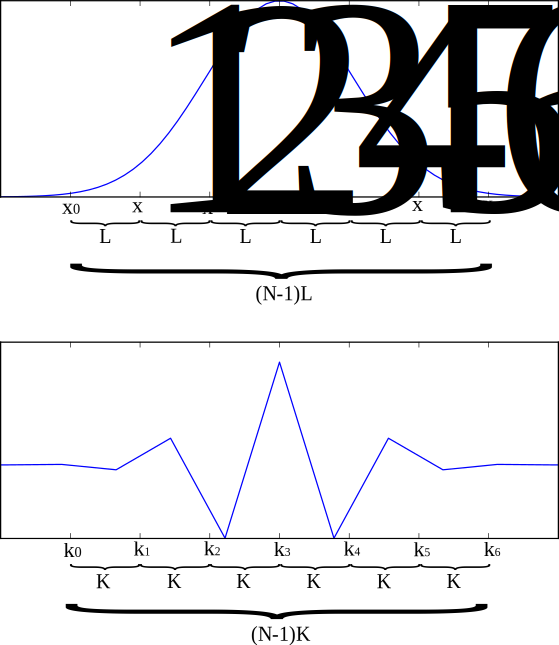
\includegraphics[width=.6\textwidth]{diagrams/fig-DFTDiagram.eps}
\caption[DFT schematic illustration.]{Schematic diagram illustrating sampling intervals and nomenclature in $x$ and $k$ domains for a DFT. In this illustration, $N=7$.
 \label{fig-DFTDiagram}}
\end{figure}
Using the relations above, the wave number samples are given by,
\begin{equation}\label{eq-fftfreq}
k_m=\frac{2\pi m}{LN}
\end{equation}
Of course, as $N$ increases, so does the accuracy of the DFT. But, in a physical problem, unlike a purely mathematical problem, the value of the $x$-component wave numbers, $k_m$, cannot exceed the wave number supported by the physical medium in which the Gaussian beam is traveling, $-k_i \leq k_m \leq k_i$. In order to achieve this, the spacial sampling interval, $L$, must remain above the minimum value given by $L\geq\lambda/2$, and N cannot increase without a corresponding increase in the size of the sampling domain. If care is taken to ensure these requirements, the DFT is effective, and can be computed very quickly with an algorithm known as the fast Fourier transform (FFT) \cite{fft}.

From this point, the process follows similarly to that outlined in the previous section. The reflection coefficients, $\tilde{r}(k_x)$ are sampled at the same $k_x$ values at which incident amplitudes are calculated, and an inverse transform is taken. It is important that the FFT algorithm can only be used to compute the inverse transform if it is also performed on the reflecting surface. If the reflected beam is to be propagated away from the surface to a detector by changing the transform kernel, the sum must be computed by other means which results in a significant increase in computation time. This is the primary weakness of the DFT method.

\subsection{Comparison of the Two Methods}
Each of the two methods above has its advantages and disadvantages, and by understanding them, the most appropriate method can be executed for each application.

The analytical method has the advantage that it can be used to propagate a reflected beam away from the boundary with no significant increase in computation time or difficulty, but it has the disadvantage that approximations must be made to the expression for the incident electric field. The most notable effect of these approximations is that the analytical Fourier transform is a strictly real function. The analytical method's second disadvantage is that the inverse transform must still be computed numerically, so numerical error will be introduced despite the approximations made.

The DFT method has the advantage of speed. The FFT algorithm makes performing the sums very fast. It also has the advantage that the only errors introduced are numerical, and consequently they can be made arbitrarily small by choosing high enough sample numbers. But its disadvantage is that the inverse transform can only be evaluated at the reflecting surface.

\begin{figure}[htb]
\centering
\includegraphics[width=\textwidth]{plots/fig-transformComparisonVariousPhi.eps}
\caption[Comparison of analytical and FFT Fourier transform methods]{Comparison of analytical and FFT Fourier transform methods for two different incident angles and Sample sizes. Significantly, the analytical transform is strictly real, leaving the curve for its imaginary part lying on axis. Also illustrated is the effect of sample number, $N$ in the FFT.
 \label{fig-transformComparisonVariousPhi}}
\end{figure}

Figure \ref{fig-transformComparisonVariousPhi} shows the Fourier transform of a Gaussian beam incident at two different angles both numerically and analytically. Note that the analytical transform is strictly real, and a continuous function, whereas the discrete transform is sampled at a finite set of points and is, in general, complex. The discrete sampling interval is different for the two incident angles, illustrating the effects of course versus fine sampling.

\begin{figure}
\centering
\includegraphics[width=.9\textheight, angle=-90]{plots/fig-surfaceReflectionProfile.eps}
\caption[Intensity profile of incident and reflected Guassian beams]{Comparison of incident and reflected intensity profile using both analytic and discrete methods. Slight pulse reshaping occurs when incidence is near the critical angle.
 \label{fig-surfaceReflectionProfile}}
\end{figure}

The differences between the analytical and FFT methods can also be seen in the surface reflection profiles they generate.  Figure \ref{fig-surfaceReflectionProfile} shows the surface profile of an incident beam in the left pane. The same incident profile plotted against the $\theta_i$ domain using both the analytical and FFT methods is shown in the center pane. The FFT spectrum shows signs of sampling effect, which could easily be eliminated by increasing the sample size. The spectra are superimposed over the reflection coefficients to depict which of the constituent plane waves are below and beyond the critical angle. The third pane shows the surface profile of the reflected beam calculated by both methods. Note that the curve for the analytical method has been scaled so the curves do not lie directly on top of one another.

\section{Finite Beam Reflection Profiles Under Many Conditions}\label{finiteBeam-variousConditions}

Having analyzed the case of a finite beam and discussed two methods to perform the relevant calculations, it will be insightful to plot the reflectivities of finite beams under various conditions. All of the graphs in this section will be computed by means of the FFT for speed considerations and because calculations at points of the reflecting surface will not need to be considered.

First I will consider a series of Gaussian beams of different waist sizes incident on a gainy reflecting surface. Figure \ref{fig-finiteBeamReflectivityP} shows $p$ polarized beams of widths between two and twelve wavelengths. The intensity vs incidence angle plot shows that the widely focused beam follows most closely to the discontinuous graph for a plane wave, while the narrowly focused beam exhibits reflectivity that increases slowly and smoothly. Figure \ref{fig-finiteBeamReflectivityS} shows the same information for $s$ polarization.

\begin{figure}[htb]
\centering
\includegraphics[width=.8\textwidth]{plots/fig-finiteBeamReflectivityP.eps}
\caption[Finite Beam Reflectivities at various spot sizes ($p$-polarization)]{Finite beam reflectivities at spot sizes of 2, 5, and 12 wavelengths ($p$ polarization). The widely focused beam follows most closely to the plane wave reflectivity.
 \label{fig-finiteBeamReflectivityP}}
\end{figure}

\begin{figure}
\centering
\includegraphics[width=.8\textwidth]{plots/fig-finiteBeamReflectivityS.eps}
\caption[Finite Beam Reflectivities at various spot sizes ($s$-polarization)]{Finite beam reflectivities at spot sizes of 2, 5, and 12 wavelengths ($s$ polarization).
 \label{fig-finiteBeamReflectivityS}}
\end{figure}

Figure \ref{fig-finiteBeamReflectivityVariousGains} holds the beam width fixed at $w_0=10\lambda$ and plots the reflectivities vs incidence angle for several values of gain, $\gamma$. Although increasing $\gamma$ to arbitrarily high values does not increase reflectivity without bound as shown in \ref{fig-gainyReflectivityFinal-highGain}, increasing gain within the realm of physically realizable values does.

\begin{figure}
\centering
\includegraphics[width=.8\textwidth]{plots/fig-finiteBeamReflectivityVariousGains.eps}
\caption[Finite Beam Reflectivities at Various Gain Factors]{Finite beam reflectivities at various gain factors, $\gamma$. Beam width fixed at $w_0=10\lambda$. At physically realizable gains, increasing $\gamma$ increases reflectivity.
 \label{fig-finiteBeamReflectivityVariousGains}}
\end{figure}

Lastly, in figure \ref{fig-finiteBeamVsGain}, reflectivity is plotted against $\gamma$ for a few incident angles. At a fixed incidence angle and spot size ($w_0=10\lambda$), it is clear that increasing gain only increases reflectivity to an extent before it falls off again. Additionally, the beam incident at $\phi=30^o$ illustrates the fact that the critical angle changes as $\gamma$ changes. The beam is incident below the critical angle at first, but as gain increases through $\gamma=0.6$, the critical angle falls below the incidence angle and the beam begins experiencing ATIR.

\begin{figure}
\centering
\includegraphics[width=.8\textwidth]{plots/fig-finiteBeamVsGain.eps}
\caption[Finite Beam Reflectivities  at a few incident angles, plotted vs $\gamma$]{Finite Beam Reflectivities  at a few incident angles, plotted vs $\gamma$. Reflectivity is bounded for a fixed incident angle, and the critical angle moves as $\gamma$ changes.
 \label{fig-finiteBeamVsGain}}
\end{figure}

%XXXXXXXXXXXXXXXXXXXXXXXXXXXXXXXXXXXXXXXXXXXXXXXXXXXXXXXXXXXXXXXXXXXX

\chapter{Conclusions}\label{chap-conclusions}
Total internal reflection has a long history of research and practical applications. Amplified total internal reflection from optically gainy media began to be studied, first experimentally and then theoretically in the 1960's. Experimental results have supported the existence of ATIR from the beginning, but difficulties in experimentally studying a single interface led to disagreement among theorists.

By analyzing in detail the case of plane waves incident on the boundary surface of both gain and loss media, this thesis claims to settle the debate about the existence of single surface amplified total internal reflection. Applying well-known boundary conditions to solutions of Maxwell's equations at the gainy or lossy surface leads to reflection coefficients for the cases of $s$ and $p$ polarization respectively given by
\begin{equation}
\tilde{r}_s=\frac{k_{iz}-\tilde{k}_{tz}}{k_{iz}+\tilde{k}_{tz}}
\end{equation}
\begin{equation}
\tilde{r}_p=\frac{\epsilon_1\tilde{k}_{tz}-\tilde{\epsilon}_2k_{iz}}{\epsilon_1\tilde{k}_{tz}+\tilde{\epsilon}_2k_{iz}}
\end{equation}

These results are agreed upon throughout the literature. The disagreement arises in choosing the value for $\tilde{k}_{tz}$. For every set of system configurations, $\tilde{k}_{tz}$ can take on one of two mathematically correct conjugate values.  Choosing the correct quadrant in the complex plane for $\tilde{k}_{tz}$ dictates whether reflectivity is amplified or attenuated.  By satisfying the following set of three conditions, the thesis shows that amplified total internal reflection occurs from gainy medium beyond the critical angle only.

\begin{enumerate}\label{conditions-conclusions}
\item A wave's amplitude must grow in the propagation direction in a gainy medium and decay in a lossy medium.
\item A non-evanescent wave behind the boundary, must propagate away from the boundary in either lossy or gainy media.
\item The solution corresponding to an evanescent wave behind the boundary, must decay away from the boundary in either lossy or gainy media.
\end{enumerate}

Because reflectivity is enhanced at incidence angles beyond the critical angle, but not below it, a discontinuous jump in reflectivity occurs at the critical angle.  This jump is surprising because so few quantities in nature exhibit discontinuities. It is significant,however, that the discontinuity is eliminated in the case of a finite width beam.

To analyze the case of a finite width beam, Fourier analysis is used to decompose an incident beam of Gaussian profile into a series of plane waves traveling in slightly different directions.  As the incidence angle of the finite beam's central ray is tuned through the critical angle, each the beam's constituent plane waves transitions through its own discontinuity one at a time such that the composite reflectivity is continuous and smooth. The reflectivity of a narrowly focused beam increases slowly and steadily as incidence angle is increased, while that of a wide beam (a better approximation of a plane wave) follows closely to the curve for a plane wave, with a sharp but still smooth rise in reflectivity near the critical angle.

Having resolved the question as to which quadrant is correct for $\tilde{k}_{tz}$, all reflectivities can be calculated by direct evaluation of the reflection coefficients above. These results are in good agreement with those of FDTD simulations run by other authors, but do not require the same computational power.


%XXXXXXXXXXXXXXXXXXXXXXXXXXXXXXXXXXXXXXXXXXXXXXXXXXXXXXXXXXXXXXXXXXXX

\bibliographystyle{plain}
%\citationstyle{} %Template said I needed this command too
\bibliography{OrndorffThesis.bib}

%XXXXXXXXXXXXXXXXXXXXXXXXXXXXXXXXXXXXXXXXXXXXXXXXXXXXXXXXXXXXXXXXXXXX
\appendix
\chapter{Source Code}
The library below is written in python and used to make all figures in this document as well as to perform the discrete Fourier transforms and numerical integrals used in analyzing Gaussian beams. It is released for free use for any purpose.  The code relies critically on the numpy, scipy, and matplotlib libraries, and couldn't have been realized without them.
\vspace{1.5em}
\singlespace
\lstinputlisting[language=Python]{plots/atir2.py}

%XXXXXXXXXXXXXXXXXXXXXXXXXXXXXXXXXXXXXXXXXXXXXXXXXXXXXXXXXXXXXXXXXXXX
\end{document}
